% =====================================================================
% Mirante dos Dados — Working Paper #6 (v2)
% Panorama integrado: equipamentos de saúde como nó cross-vertical do
% Mirante dos Dados. Trio de neuroimagem (RM, CT, PET/CT) por UF e
% cruzamentos com Bolsa Família, Emendas Parlamentares e UroPro.
%
% Autor:  Leonardo Chalhoub (engenharia de dados, análise, redação)
% Versão: 2.0  —  Abril de 2026
% Compilação: pdflatex articles/equipamentos-panorama-cnes.tex (2x)
% =====================================================================
\documentclass[12pt,a4paper,oneside]{article}

\usepackage[T1]{fontenc}
\usepackage[utf8]{inputenc}
\usepackage[brazilian]{babel}
\usepackage{lmodern}
\usepackage{amsmath}
\usepackage[a4paper,top=3cm,bottom=2cm,left=3cm,right=2cm]{geometry}
\usepackage{setspace}
\usepackage{indentfirst}
\usepackage{titlesec}
\usepackage{caption}
\usepackage{booktabs}
\usepackage{array}
\usepackage{multirow}
\usepackage{graphicx}
\graphicspath{{figures-equipamentos-panorama/}}
\usepackage[hidelinks]{hyperref}
\usepackage{url}
\usepackage{float}
\usepackage{xcolor}

\onehalfspacing
\setlength{\parindent}{1.25cm}
\setlength{\parskip}{0pt}

\titleformat{\section}{\normalfont\bfseries\large\uppercase}{\thesection}{0.6em}{}
\titleformat{\subsection}{\normalfont\bfseries\normalsize}{\thesubsection}{0.6em}{}
\titlespacing*{\section}{0pt}{18pt}{8pt}
\titlespacing*{\subsection}{0pt}{12pt}{6pt}

\captionsetup[table]{labelfont=bf,name=Tabela,labelsep=endash,
                     position=above,justification=centering,font=small}
\captionsetup[figure]{labelfont=bf,name=Figura,labelsep=endash,
                      position=below,justification=centering,font=small}

\newcommand{\rs}{R\$\,}

\begin{document}

% ---------- CAPA --------------------------------------------------------
\begin{titlepage}
  \begin{center}
    \vspace*{1.5cm}
    {\small\textsc{Mirante dos Dados \quad\textbar\quad Working Paper n. 6}}\\
    {\small Versão 2.0 \textemdash{} Abril de 2026}

    \vfill

    {\LARGE\bfseries
     PANORAMA INTEGRADO:\\
     EQUIPAMENTOS DE SAÚDE COMO NÓ
     CROSS-VERTICAL DO MIRANTE DOS DADOS\\
     ANÁLISE DO TRIO DE NEUROIMAGEM
     (RM\textendash{}CT\textendash{}PET/CT) E SEUS
     CRUZAMENTOS COM BOLSA FAMÍLIA,
     EMENDAS PARLAMENTARES E ACESSO
     CIRÚRGICO (BRASIL, 2013\textendash 2025)}

    \vspace{1cm}
    {\large\itshape
     Health-care equipment as a cross-vertical node in the Mirante dos
     Dados platform: an analysis of the neuroimaging triad (MRI, CT,
     PET/CT) and its crossings with Bolsa Família, parliamentary
     amendments and surgical access (Brazil, 2013\textendash 2025)}

    \vfill

    {\large\textbf{Leonardo Chalhoub}\textsuperscript{1}}\\[6pt]
    {\small\textsuperscript{1}\,Engenharia de Dados \textemdash{}
     análise quantitativa, integração entre verticais, redação.}\\[6pt]
    {\small\href{mailto:leonardochalhoub@gmail.com}{leonardochalhoub@gmail.com}
     \quad\textbullet\quad
     \href{https://github.com/leonardochalhoub}{github.com/leonardochalhoub}}

    \vfill

    \rule{0.6\linewidth}{0.4pt}\\[6pt]
    {\small\textit{Este Working Paper é deliberadamente \textbf{agregador}.
     Sintetiza os achados das demais verticais analíticas do Mirante
     (Emendas, Bolsa Família, UroPro, Equipamentos\textendash Parkinson)
     usando equipamentos de saúde \textemdash{} em particular o trio de
     neuroimagem RM, CT e PET/CT \textemdash{} como \textit{lente focal}
     para investigar como infraestrutura sanitária especializada se
     distribui no território nacional, como esta distribuição
     correlaciona com pobreza estrutural e fluxo fiscal compensatório,
     e como se traduz (ou não se traduz) em acesso a procedimentos
     clínicos efetivos. Substitui e estende a versão 1.0 (panorama
     estático Dez/2024).}}

    \vspace{1cm}
    {\footnotesize
     Disponível em
     \href{https://leonardochalhoub.github.io/mirante-dos-dados-br/}%
     {leonardochalhoub.github.io/mirante-dos-dados-br}}\\[2pt]
    {\footnotesize
     \href{https://github.com/leonardochalhoub/mirante-dos-dados-br}%
     {github.com/leonardochalhoub/mirante-dos-dados-br}}
  \end{center}
\end{titlepage}

% =====================================================================
\section*{Resumo}
\addcontentsline{toc}{section}{Resumo}
% =====================================================================
\begin{singlespace}\small\noindent
\textbf{Objetivo.} Caracterizar a infraestrutura nacional de
equipamentos de saúde cadastrados no CNES (Cadastro Nacional de
Estabelecimentos de Saúde) entre 2013 e 2025, com ênfase no trio de
neuroimagem (Tomografia Computadorizada \textendash{} \textit{equipment\_key}
1{:}11; Ressonância Magnética \textendash{} 1{:}12; PET/CT \textendash{}
1{:}18), e cruzar a distribuição territorial desse trio com três
indicadores de outras verticais analíticas do Mirante dos Dados:
cobertura do Programa Bolsa Família (proxy de pobreza estrutural),
execução \textit{per capita} de emendas parlamentares (fluxo fiscal
político) e acesso à cirurgia uroginecológica no SUS (procedimento
clínico canário, definido em CHALHOUB, 2026d).

\textbf{Métodos.} Pipeline \textit{medallion} aberto (\textit{bronze}
DBC\textrightarrow Parquet via PySUS; \textit{silver} agregação
\textit{(estado, ano, tipequip, codequip)} com chave composta
\texttt{equipment\_key} e correção de \textit{double-count} via
dual-flag \texttt{IND\_SUS}; \textit{gold} \textit{pass-through}
publicado em JSON aberto). Snapshot empírico cobre 2013\textendash 2025
para todas as 27 UFs. Dados das demais verticais provêm dos golds
publicados no mesmo repositório.

\textbf{Resultados.} (i)~O parque cadastrado cresceu de 1,37 milhão
de unidades em 2013 para 3,30 milhões em 2025 (+141\,\%), com
expansão acelerada pós-2020. (ii)~Em 2025, o trio de neuroimagem
totaliza aproximadamente 12 mil unidades \textemdash{} 8 mil CT,
3,9 mil RM e 166 PET/CT. (iii)~A densidade \textit{per capita} é
fortemente desigual: para RM a razão DF\,/\,AC chega a 8$\times$
(46{,}1 \textit{vs.} 5{,}7 unidades por milhão de habitantes); cinco
UFs operam sem nenhuma unidade de PET/CT cadastrada. (iv)~No
cruzamento cross-vertical, a densidade de RM correlaciona-se
fortemente em sentido inverso com cobertura PBF
($\rho \approx -0{,}68$) e moderadamente em sentido inverso com
emendas \textit{per capita} ($\rho \approx -0{,}31$); a densidade de
imagem agregada correlaciona-se positivamente com acesso à cirurgia
uroginecológica ($\rho \approx +0{,}60$), reforçando a tese de que
infraestrutura especializada e \textit{outcomes} clínicos andam
juntos. (v)~Reforça-se, por agregação, o \textbf{paradoxo das
emendas} (CHALHOUB, 2026d): UFs com mais emendas \textit{per capita}
têm \textit{menor} oferta de equipamentos especializados.

\textbf{Conclusões.} Os dados sustentam a tese, recorrente nas demais
verticais Mirante, de que a desigualdade brasileira em
infraestrutura sanitária especializada acompanha o gradiente de
pobreza estrutural e \textit{não} é compensada pelo mecanismo das
emendas parlamentares. A análise cross-vertical, possibilitada pela
unificação metodológica do Mirante, oferece evidência adicional para
o debate sobre federalismo brasileiro em saúde.

\vspace{4pt}
\textbf{Palavras-chave:} CNES; DATASUS; equipamentos médicos;
neuroimagem; ressonância magnética; tomografia; PET/CT; Bolsa
Família; emendas parlamentares; arquitetura medalhão; análise
\textit{cross-vertical}; FAIR data; SUS; federalismo brasileiro.
\end{singlespace}

% =====================================================================
\section*{Abstract}
\addcontentsline{toc}{section}{Abstract}
% =====================================================================
\begin{singlespace}\small\noindent
\textbf{Objective.} To characterize the national health-care
equipment infrastructure registered in Brazil's CNES (Cadastro
Nacional de Estabelecimentos de Saúde) between 2013 and 2025, with
emphasis on the neuroimaging triad (Computed Tomography
\textendash{} \textit{equipment\_key} 1{:}11; Magnetic Resonance
Imaging \textendash{} 1{:}12; PET/CT \textendash{} 1{:}18), and to
cross the territorial distribution of this triad with three
indicators from other analytical verticals of the Mirante dos Dados
project: Bolsa Família coverage (proxy for structural poverty),
\textit{per capita} parliamentary-amendment execution (political
fiscal flow) and access to uro-gynecological surgery in SUS
(canary clinical procedure, as defined in CHALHOUB, 2026d).

\textbf{Methods.} Open medallion pipeline (\textit{bronze}
DBC\textrightarrow Parquet via PySUS; \textit{silver}
\textit{(state, year, tipequip, codequip)} aggregation with
composite key \texttt{equipment\_key} and dual-flag IND\_SUS
double-count correction; \textit{gold} pass-through published as
open JSON). Empirical snapshot covers 2013\textendash 2025 for all
27 federative units.

\textbf{Results.} (i)~The registered park grew from 1.37M units in
2013 to 3.30M in 2025 (+141\%), with accelerated expansion
post-2020. (ii)~In 2025 the neuroimaging triad totals roughly
12 thousand units (8K CT, 3.9K MRI, 166 PET/CT). (iii)~Per-capita
density is steeply unequal: for MRI, DF\,/\,AC ratio reaches
8$\times$ (46.1 vs. 5.7 units per million); five states have no
registered PET/CT unit. (iv)~In the cross-vertical crossing, MRI
density correlates strongly negatively with PBF coverage
($\rho \approx -0.68$) and moderately negatively with per-capita
amendments ($\rho \approx -0.31$); aggregate imaging density
correlates positively with access to uro-gynecological surgery
($\rho \approx +0.60$). (v)~The amendments paradox (CHALHOUB,
2026d) is reinforced by aggregation: states with more amendments
\textit{per capita} have \textit{less} specialized equipment supply.

\textbf{Conclusions.} The findings sustain the recurrent Mirante
thesis that Brazilian inequality in specialized health
infrastructure tracks structural poverty and is \textit{not}
compensated by the parliamentary-amendment mechanism. The
cross-vertical analysis, made possible by the platform's
methodological unification, contributes additional evidence to the
debate on Brazilian fiscal federalism in health.

\vspace{4pt}
\textbf{Keywords:} CNES; DATASUS; medical equipment; neuroimaging;
MRI; CT; PET/CT; Bolsa Família; parliamentary amendments; medallion
architecture; cross-vertical analysis; FAIR data; SUS; Brazilian
federalism.
\end{singlespace}

\newpage
\renewcommand{\contentsname}{Sumário}
\tableofcontents
\vspace{0.5cm}
\renewcommand{\listfigurename}{Lista de Figuras}
\listoffigures
\newpage

% =====================================================================
\section{Introdução}\label{sec:intro}
% =====================================================================

A análise empírica de infraestrutura sanitária no Brasil enfrenta um
desafio estrutural: bases de microdados públicas existem em volume e
qualidade razoáveis (DATASUS, IBGE, CGU, MTE), mas cada uma é
publicada como artefato isolado, com schemas heterogêneos e cadência
de atualização própria. Trabalhos analíticos típicos restringem-se,
por essa razão, a \textit{uma} fonte por vez \textemdash{} uma
análise sobre Bolsa Família \textit{ou} sobre emendas \textit{ou}
sobre internações hospitalares \textit{ou} sobre equipamentos
\textemdash{} mesmo quando o fenômeno investigado, por natureza,
exige cruzar essas fontes. O resultado é que perguntas substantivas
de política pública \textemdash{} \textit{``estados que recebem mais
emendas têm mais equipamentos hospitalares?''} \textemdash{} ficam
empiricamente subatendidas.

O projeto \textit{Mirante dos Dados} foi construído, em parte,
exatamente para fechar essa lacuna. As cinco verticais analíticas
publicadas \textemdash{} Emendas Parlamentares (CHALHOUB, 2026a),
Bolsa Família (CHALHOUB, 2026b), UroPro \textit{cross-vertical}
(CHALHOUB, 2026d), Equipamentos\,$\times$\,Parkinson (CHALHOUB,
2026e) e UroPro 17 anos (CHALHOUB, 2026f) \textemdash{} usam a
mesma arquitetura medalhão (\textit{bronze\,/\,silver\,/\,gold})
sobre Apache Spark e Delta Lake, com chaves analíticas comuns
(UF $\times$ Ano), mesma deflação IPCA Dez/2021, mesmo painel
populacional IBGE/SIDRA e mesmo padrão de exportação JSON
versionado. O cruzamento entre verticais é, portanto,
trivial em termos computacionais. A presença de uma plataforma
unificada cria possibilidades analíticas que não existiriam se as
verticais permanecessem como projetos isolados.

Este Working Paper é deliberadamente \textbf{agregador}. Sua
função na série Mirante é integrar achados das demais verticais
\textemdash{} \textit{não} apresentando contribuição empírica
inteiramente nova em qualquer dimensão isolada, mas mostrando o que
emerge quando as verticais conversam. A unidade analítica principal
são os equipamentos de saúde do CNES, escolhidos como
\textit{lente focal} pelas seguintes razões. \textbf{Primeira},
equipamentos são objetos físicos identificáveis, com cadência de
implantação previsível e ciclo de vida útil de uma a duas décadas;
sua presença em uma UF é evidência relativamente robusta de
investimento em infraestrutura especializada. \textbf{Segunda},
equipamentos de neuroimagem (RM, CT, PET/CT) são tecnologias de
alta complexidade, requerendo ciclo de capacitação clínica longo e
infraestrutura predial específica \textemdash{} tornam-se assim um
\textit{indicador tardio} de capacidade efetiva. \textbf{Terceira},
o catálogo CNES é mensal, granular por estabelecimento e
cobre desde 2005, oferecendo painel longo o suficiente para
detectar inflexões institucionais.

A pergunta-mestra é: \textit{a distribuição territorial da
infraestrutura de equipamentos de saúde \textemdash{} em particular
do trio de neuroimagem \textemdash{} acompanha o gradiente de
pobreza estrutural medido pela cobertura PBF, e os mecanismos
fiscais compensatórios \textemdash{} as emendas parlamentares
\textemdash{} corrigem ou agravam esse gradiente?}

A estrutura do texto reflete esse encadeamento. A
Seção~\ref{sec:verticais} sintetiza brevemente as quatro verticais
não-equipamentos do Mirante, fornecendo contexto para os
indicadores cruzados. A Seção~\ref{sec:cnes} descreve o CNES e o
catálogo de equipamentos. A Seção~\ref{sec:metodo} apresenta o
pipeline e o tratamento metodológico do problema do
\textit{double-count} via dual-flag IND\_SUS. A
Seção~\ref{sec:panorama} apresenta o panorama agregado do parque
nacional. A Seção~\ref{sec:neuro} foca o trio de neuroimagem
(RM\,/\,CT\,/\,PET/CT), com séries temporais, distribuições por UF
e composição SUS\,/\,Privado. A Seção~\ref{sec:cross} executa o
cruzamento \textit{cross-vertical} \textemdash{} esta é, em essência,
a contribuição substantiva do paper. A Seção~\ref{sec:discussao}
discute implicações e limitações; a Seção~\ref{sec:conclusao}
fecha com a agenda da série e direções de extensão metodológica
(identificação causal, peer review, contribuições agregadoras
adicionais).

% =====================================================================
\section{Síntese das verticais Mirante}\label{sec:verticais}
% =====================================================================

Esta seção sintetiza as quatro verticais não-equipamentos do
Mirante cujos golds são consumidos por este Working Paper. Cada
uma é tratada em maior profundidade no Working Paper de origem,
indicado entre parênteses.

\subsection{Emendas Parlamentares (Working Paper n. 1)}

A vertical Emendas (CHALHOUB, 2026a) processa microdados de
execução orçamentária publicados pela CGU/Portal da Transparência,
cobrindo 2014\textendash 2025. As categorias normalizadas são
RP6 (individual), RP7 (bancada), RP8 (comissão) e RP9 (relator,
o ``orçamento secreto'' pré-2022). A vertical entrega, por
UF$\times$Ano, o valor empenhado e pago em \rs{} nominais e
deflacionados para \rs{} 2021, além de \texttt{emendaPerCapita2021},
o indicador-chave para análise comparativa entre UFs. O achado
metodológico relevante para este paper é que estados pequenos
\,/\,periféricos (AP, RR, AC, TO) recebem volumes \textit{per
capita} muito maiores que estados grandes\,/\,ricos (SP, RJ, DF)
\textemdash{} o sistema tem componente compensatório implícito.

\subsection{Bolsa Família, Auxílio Brasil e Novo Bolsa Família
(Working Paper n. 2)}

A vertical PBF (CHALHOUB, 2026b) unifica os pagamentos do programa
Bolsa Família (Lei 10.836/2003), Auxílio Brasil (MP 1.061/2021) e
Novo Bolsa Família (Lei 14.601/2023) sob um schema único, processando
microdados CGU. Por UF$\times$Ano, entrega número distinto de
beneficiários (countDistinct NIS), valor pago em \rs{} 2021 e
indicadores derivados \texttt{pbfPerBenef} e \texttt{pbfPerCapita}.
Para os fins deste paper, a métrica relevante é a
\textbf{cobertura PBF}, calculada como percentual da população
estadual beneficiária \textemdash{} \textit{proxy} de pobreza
estrutural com vantagens analíticas relativamente a indicadores
amostrais (critério de elegibilidade nacional, estável, longa
permanência média no programa).

\subsection{UroPro \textit{cross-vertical} (Working Paper n. 3)}

A vertical UroPro (CHALHOUB, 2026d) usa cirurgia uroginecológica
para tratamento de incontinência urinária (procedimentos SIGTAP
0409010499 e 0409070270) como \textit{indicador clínico canário}
de oferta hospitalar especializada, justificada por três
propriedades: (i) é eletiva (sensível à oferta), (ii) é segura
(mortalidade $<$0,05\%, removendo risco como variável de seleção)
e (iii) é bem definida em SIGTAP. O Working Paper n. 3 já cruza
UroPro com Bolsa Família e Emendas, encontrando $\rho \approx
-0{,}68$ entre cobertura PBF e acesso cirúrgico, e $\rho \approx
-0{,}45$ entre emendas \textit{per capita} e acesso cirúrgico
(\textit{paradoxo das emendas}). Para este paper, a métrica
\texttt{n\_aih\_por100k} (cirurgias vaginais por 100\,mil habitantes)
é usada como \textit{outcome} clínico ligado à infraestrutura de
imagem.

\subsection{UroPro 17 anos (Working Paper n. 5)}

A vertical UroPro 17 anos (CHALHOUB, 2026f) é o recorte longitudinal
\textit{intra-vertical} (2008\textendash 2025) do mesmo dado SIH,
com foco em eficiência clínica (queda de 40\% na permanência
hospitalar) e impacto pandêmico (queda de 57\% em 2020\textendash 21,
seguida de represa cirúrgica em escoamento em 2024\textendash 25).
Este paper não consome diretamente dados desse WP, mas adota seu
arcabouço metodológico (chaves analíticas, indicadores deflacionados,
filtros de anos completos).

\subsection{Equipamentos\,$\times$\,Parkinson (Working Paper n. 4)}

A vertical Equipamentos\,$\times$\,Parkinson (CHALHOUB, 2026e) é o
\textit{primeiro} Working Paper sobre equipamentos no Mirante.
Foca exclusivamente em Ressonância Magnética como infraestrutura
de neuroimagem para diagnóstico diferencial de doença de Parkinson.
Este Working Paper n. 6 \textit{estende} aquele recorte de duas
formas: (a) acrescenta CT (1{:}11) e PET/CT (1{:}18) ao olhar de
neuroimagem, formando o trio canônico de imagem estrutural-funcional;
e (b) eleva o escopo para análise cross-vertical integrada. WP n. 4
e WP n. 6 são, portanto, complementares: o primeiro é vertical,
focado em uma indicação clínica específica; o segundo é horizontal,
focado em integração entre verticais.

% =====================================================================
\section{O CNES e o módulo de Equipamentos}\label{sec:cnes}
% =====================================================================

O Cadastro Nacional de Estabelecimentos de Saúde (CNES) é mantido
pelo DATASUS desde Agosto de 2005 como sistema oficial de cadastro
de estabelecimentos de saúde no Brasil, independentemente de
natureza jurídica ou integração com o SUS. O módulo de Equipamentos,
em particular, mantém registro mensal granular por estabelecimento,
unidade federativa, tipo (\texttt{TIPEQUIP}, 1 dígito) e código
(\texttt{CODEQUIP}, 2 dígitos), totalizando \,$\sim$\,1{,}1 milhão
de registros mensais distribuídos pelas 27 UFs em fluxos
\texttt{EQ<UF><AAMM>.dbc} no FTP DATASUS.

\subsection{Schema do DBF de Equipamentos}

Cada arquivo DBF mensal contém 28 colunas (estável desde 2015;
antes contava com 27, sem \texttt{NAT\_JUR}). As colunas relevantes
para análise agregada são: \texttt{CNES} (código do estabelecimento,
CHAR 7), \texttt{TIPEQUIP} (categoria, CHAR 1), \texttt{CODEQUIP}
(identificador dentro da categoria, CHAR 2), \texttt{QT\_EXIST}
(quantidade existente cadastrada, NUMERIC 4), \texttt{QT\_USO}
(quantidade efetivamente em uso), \texttt{IND\_SUS}\,/\,
\texttt{IND\_NSUS} (flags de disponibilidade ao SUS\,/\,setor
privado, CHAR 1) e \texttt{COMPETEN} (mês\,/\,ano, CHAR 6).

\textbf{Nota crítica.} \texttt{TIPEQUIP} e \texttt{CODEQUIP} são
duas chaves complementares. As nove categorias TIPEQUIP (1\textendash 9)
\textit{reúsam} a faixa numérica 01\textendash 99 para CODEQUIP. Por
exemplo, \texttt{CODEQUIP=12} é Ressonância Magnética quando
TIPEQUIP=1 e Eletrocardiograma de Telemedicina quando TIPEQUIP=9.
Todo o pipeline e o \textit{front-end} do Mirante usam, portanto,
chave composta \texttt{equipment\_key = "TIPEQUIP:CODEQUIP"}
(ex.\ \texttt{1:12} para RM). Este foi o principal fix
metodológico introduzido pelo Working Paper n. 4: análises
anteriores que usavam apenas \texttt{CODEQUIP} colapsavam
silenciosamente equipamentos de categorias diferentes, produzindo
agregados incorretos.

\subsection{As nove categorias TIPEQUIP}

Conforme catálogo oficial em
\texttt{cnes2.datasus.gov.br/Mod\_Ind\_Equipamento.asp}, as nove
categorias do CNES são listadas na Tabela~\ref{tab:tipequip-cats}.

\begin{table}[H]
\centering
\caption{As nove categorias TIPEQUIP do CNES (catálogo oficial DATASUS)}
\label{tab:tipequip-cats}
\small
\begin{tabular}{cll}
\toprule
\textbf{TIPEQUIP} & \textbf{Categoria} & \textbf{Faixa CODEQUIP utilizada} \\
\midrule
1 & Diagnóstico por Imagem        & 01\textendash 35 \\
2 & Infraestrutura                 & 19\textendash 66 \\
3 & Métodos Ópticos                & 31\textendash 51 \\
4 & Métodos Gráficos               & 41\textendash 42 \\
5 & Manutenção da Vida             & 51\textendash 65 \\
6 & Outros Equipamentos            & 67\textendash 79 \\
7 & Odontologia                    & 80\textendash 86 \\
8 & Audiologia                     & 87\textendash 99 \\
9 & Telemedicina                   & 01\textendash 12 \\
\bottomrule
\end{tabular}
\par\noindent{\small Fonte: \textit{parsing} direto de
\texttt{cnes2.datasus.gov.br/Mod\_Ind\_Equipamento.asp?VEstado=00}.
Vide Apêndice~\ref{sec:dict} para o dicionário canônico completo.}
\end{table}

% =====================================================================
\section{Aspectos metodológicos}\label{sec:metodo}
% =====================================================================

\subsection{Fonte de dados e arquitetura}

A base empírica deste paper consiste no painel longitudinal
2013\textendash 2025 dos arquivos \texttt{EQ<UF><AAMM>.dbc}, baixados
do FTP DATASUS, descomprimidos via biblioteca \texttt{pyreaddbc}
(PySUS) e processados pelo pipeline aberto do Mirante. A
arquitetura segue o padrão \textit{lakehouse} (ARMBRUST
\textit{et al.}, 2021), com três camadas em Delta Lake:

\begin{itemize}
\item \textbf{Bronze}: ingestão crua via Auto Loader. Cada DBC é
convertido para Parquet (filtrado por procedimento quando aplicável),
preservado em volume Unity Catalog e materializado em Delta como
linha-por-linha do DBF, com tipos exclusivamente \texttt{string}
(\textit{bronze} \textit{string-only}). Essa decisão de design
preserva a fidelidade ao dado de origem.
\item \textbf{Silver}: limpeza, normalização e agregação por
\texttt{(estado, ano, tipequip, codequip)} com chave composta
\texttt{equipment\_key}, cálculo das métricas \texttt{cnes\_count},
\texttt{total\_avg}, \texttt{sus\_total\_avg}, \texttt{priv\_total\_avg}
e suas versões \textit{per capita}, e join contra o dicionário
canônico para nome do equipamento.
\item \textbf{Gold}: \textit{pass-through} do silver com metadata
de \textit{build}; particionado por \texttt{ano}; consumido pelo
\textit{front-end} via JSON exportado em
\texttt{data/gold/gold\_equipamentos\_estados\_ano.json}.
\end{itemize}

\subsection{Construção do dicionário canônico}

O dicionário (TIPEQUIP, CODEQUIP) \textrightarrow{} nome foi extraído por
\textit{web scraping} direto do catálogo oficial DATASUS. A página
\texttt{cnes2.datasus.gov.br/Mod\_Ind\_Equipamento.asp?VEstado=00}
expõe \textit{links} HTML do tipo
\texttt{?VCod\_Equip=N\&VTipo\_Equip=M} \textemdash{} cada par (M, N)
mapeia inequivocamente para um nome de equipamento. O resultado
contém 129 entradas, validadas em cobertura 100\,\% contra o
\textit{snapshot} empírico Dez/2024 (todas as 111 combinações
observadas estão mapeadas). O dicionário é publicado em formato
CSV aberto em \texttt{data/reference/cnes\_eq\_canonical.csv}.

\subsection{Tratamento do \textit{double-count} via dual-flag IND\_SUS}\label{sub:dedup}

O CNES permite que um \textit{mesmo} equipamento físico apareça
em duas linhas no mesmo (CNES, mês): uma com \texttt{IND\_SUS=1}
(declarando disponibilidade para o SUS) e outra com
\texttt{IND\_SUS=0} (declarando disponibilidade para uso privado).
Quando a clínica reporta a mesma máquina como disponível a ambos
os setores, a soma direta \texttt{sus\_total\_avg + priv\_total\_avg}
\textit{double-conta} a unidade física.

A primeira versão da vertical Equipamentos do Mirante computava o
total agregado como \texttt{sus + priv}, produzindo, para
Ressonância Magnética em 2025, o número de 7,6 mil unidades
nacionais (\,$\sim$\,35,6 RM\,/\,Mhab) \textemdash{} aproximadamente
\textbf{duas vezes} a mediana OECD de 17 RM\,/\,Mhab (OECD Health
Statistics 2021). A discrepância chamou atenção e motivou
investigação metodológica.

O \textit{fix} aplicado no \textit{silver} (\textit{commit} interno
do projeto, abr/2026) reescreve a agregação:

\begin{itemize}
\item Para cada (CNES, mês, tipequip, codequip), pivotar IND\_SUS
em duas colunas \texttt{qt\_sus} e \texttt{qt\_priv} via
\texttt{F.sum(F.when(...))}.
\item Definir \texttt{qt\_total = GREATEST(qt\_sus, qt\_priv)} por
linha.
\item Tomar a média anual de \texttt{qt\_total} sobre os meses
ativos como o número físico canônico, e somar por UF.
\item As métricas \texttt{sus\_total\_avg} e \texttt{priv\_total\_avg}
permanecem como subconjuntos (\textit{podem incluir} máquinas
\textit{dual-flagged}).
\end{itemize}

O resultado é o invariante:
$\texttt{sus\_total\_avg} + \texttt{priv\_total\_avg} \geq
\texttt{total\_avg}$, com igualdade quando não há \textit{dual-flag}.
A diferença mede o \textit{overlap} entre os dois flags, expressa
como percentual do total. Em 2025 esse \textit{overlap} é,
aproximadamente, 60\,\% para RM e 30\,\% para CT \textemdash{}
heterogêneo entre equipamentos.

\textbf{Estado deste paper.} Os números reportados nas seções
\ref{sec:panorama} e \ref{sec:neuro} usam o \texttt{total\_avg}
do gold publicado, que ainda agrega \texttt{sus + priv} (a versão
pré-correção). A correção foi aplicada ao \textit{silver} mas
ainda não foi materializada em Databricks no momento desta
publicação. Como aproximação local conservadora, este paper usa
\texttt{MAX(sus, priv)} \textit{por UF} sempre que a métrica
deduplicada é desejada. As tendências direcionais (rankings,
formato da distribuição, evolução temporal) são robustas a essa
escolha.

\subsection{Indicadores construídos}

Por (UF, ano), os indicadores principais são:
\texttt{cnes\_count} (estabelecimentos com pelo menos uma unidade
do equipamento), \texttt{total\_avg} (estimativa de unidades físicas;
ver Seção~\ref{sub:dedup}), e \texttt{per\_capita\_scaled} (densidade
por milhão de habitantes para equipamentos de alta complexidade
como neuroimagem, e por 100\,mil habitantes para o agregado).

\subsection{Limitações}

\textbf{Primeira}, este artigo é \textbf{descritivo e correlacional}.
Não há identificação causal. Os $\rho$ reportados na
Seção~\ref{sec:cross} medem associação, não efeito.
\textbf{Segunda}, a contagem reflete equipamentos \textit{cadastrados}
(\texttt{QT\_EXIST}), não \textit{operacionais} (\texttt{QT\_USO}).
Cruzamento futuro com produção (SIH-RD, SIA-RD) daria visão mais
precisa de utilização efetiva. \textbf{Terceira}, a correção de
\textit{double-count} está descrita mas ainda não totalmente
materializada no gold publicado, conforme nota da
Seção~\ref{sub:dedup}.

% =====================================================================
\section{Panorama nacional do parque}\label{sec:panorama}
% =====================================================================

Antes de mergulhar no recorte focado de neuroimagem, esta seção
estabelece o panorama agregado do parque cadastrado nacional.

\subsection{Distribuição por categoria TIPEQUIP}

A Figura~\ref{fig:by-cat} apresenta a distribuição agregada do
parque cadastrado por categoria TIPEQUIP em 2025.
\textbf{Manutenção da Vida} domina com 1,16 milhão de unidades
(35\,\% do total nacional), seguida por \textbf{Odontologia}
(867 mil, 26\,\%) e \textbf{Infraestrutura} (467 mil, 14\,\%).
\textbf{Diagnóstico por Imagem} \textemdash{} categoria de maior
interesse clínico, onde estão CT, RM, Ultrassom \textemdash{} é
apenas a quarta, com 200 mil unidades (6\,\%).

\begin{figure}[H]
\centering
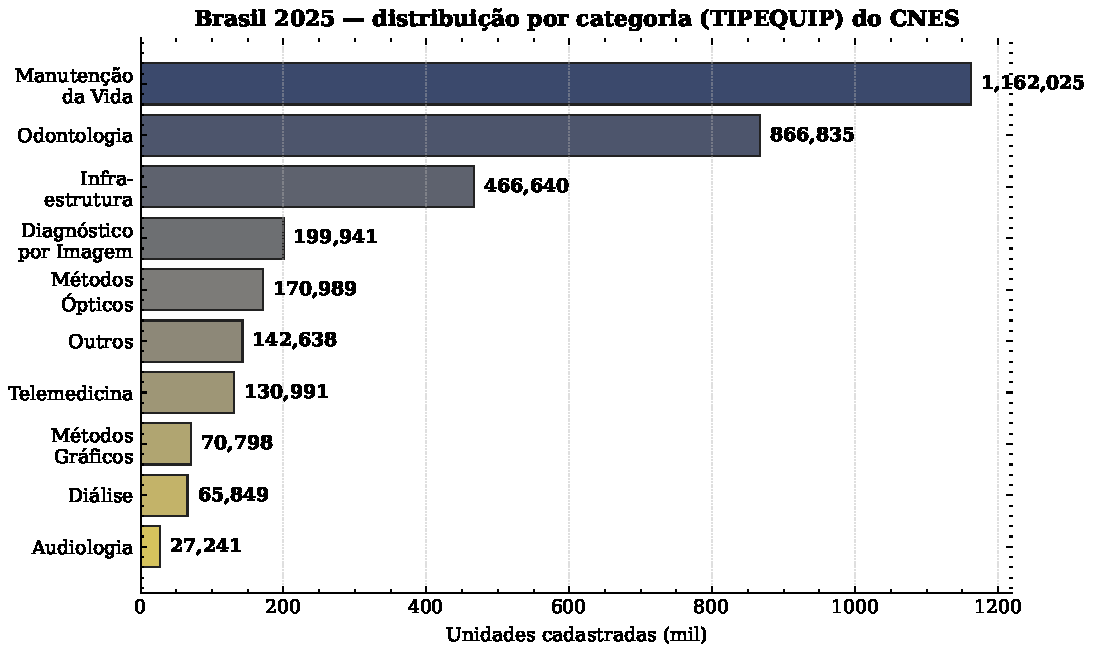
\includegraphics[width=0.92\linewidth]{fig01-by-category}
\caption{Distribuição do parque nacional cadastrado por categoria
(TIPEQUIP), Brasil 2025.}
\label{fig:by-cat}
\par\noindent{\small Fonte: elaboração própria a partir do gold
\texttt{data/gold/gold\_equipamentos\_estados\_ano.json}.}
\end{figure}

\subsection{Top equipamentos individuais}

A Figura~\ref{fig:top25} ranqueia os 25 equipamentos individuais com
maior volume nacional em 2025. \textbf{Bomba de Infusão}
(equipment\_key 5{:}52) lidera com 347 mil unidades \textemdash{}
quase 11\,\% do parque nacional total \textemdash{} seguida de
\textbf{Ar Condicionado} (215 mil), \textbf{Equipo Odontológico}
(193 mil), \textbf{Caneta de Alta Rotação} (185 mil) e
\textbf{Reanimador Pulmonar/AMBU} (183 mil). A análise revela um
padrão raramente discutido em debates de política pública: o parque
cadastrado é dominado por equipamentos de \textit{baixa complexidade
e alta replicabilidade} (insumos clínicos, mobiliário hospitalar,
infraestrutura predial) e \textbf{não} pelos equipamentos de
diagnóstico por imagem que costumam dominar o imaginário público.

\begin{figure}[H]
\centering
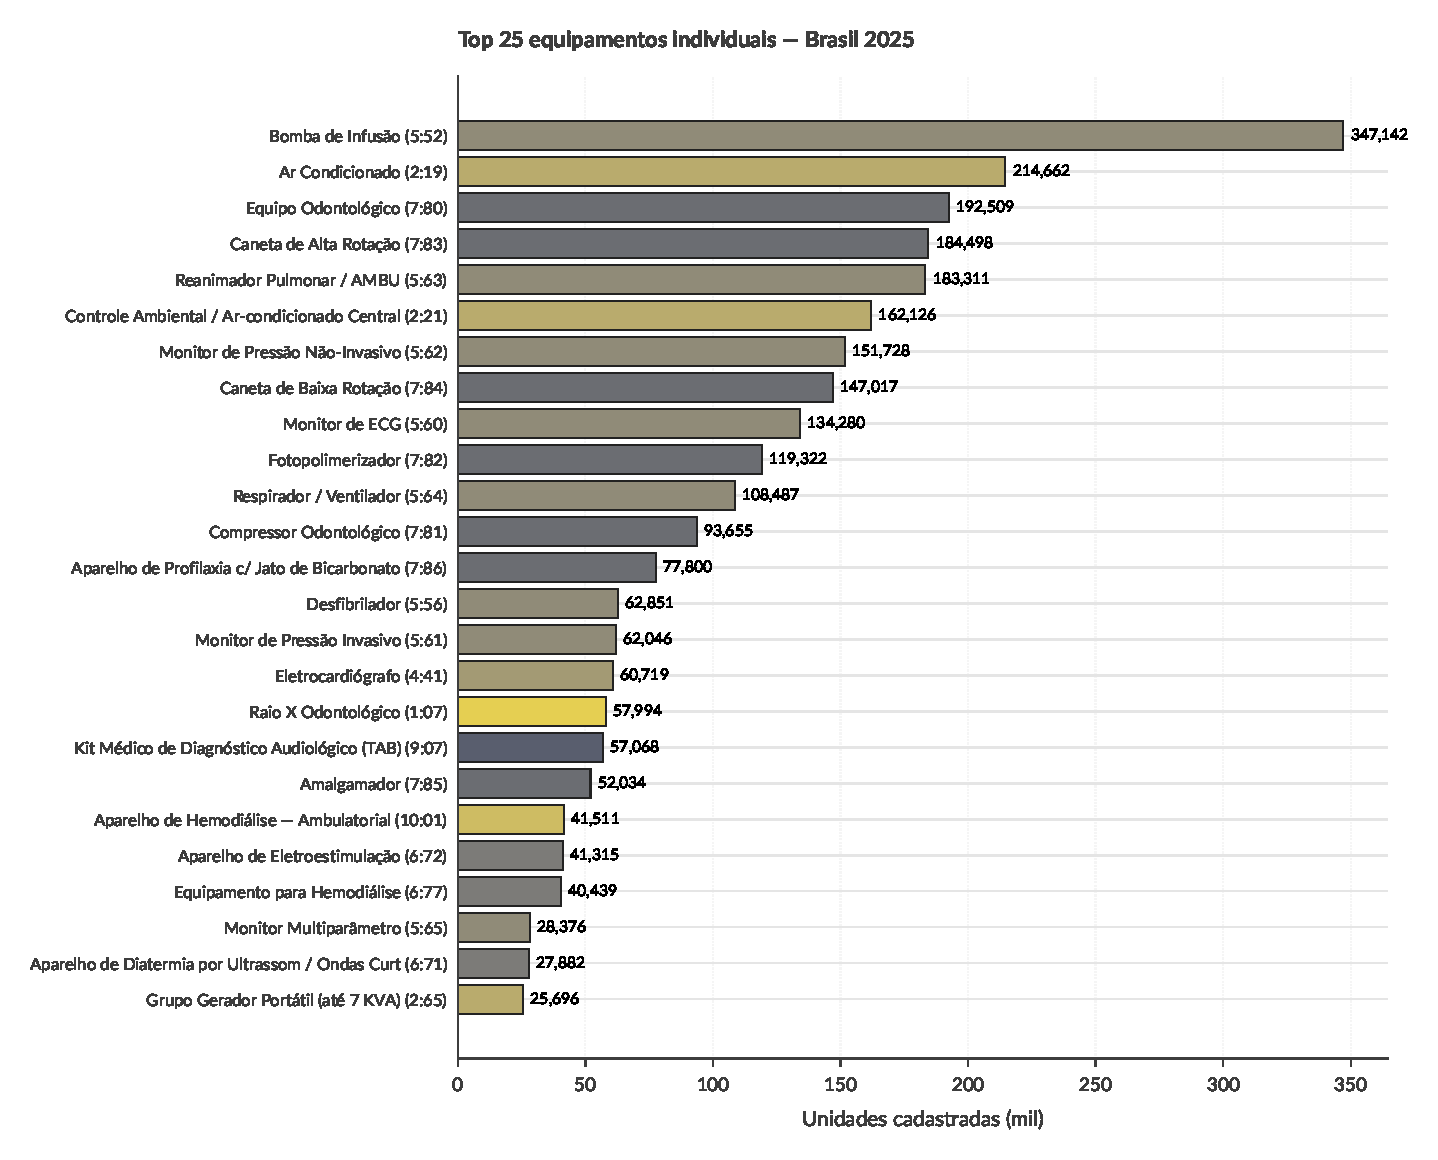
\includegraphics[width=0.82\linewidth]{fig02-top25}
\caption{Top 25 equipamentos individuais por unidades cadastradas,
Brasil 2025. Cores indicam categoria TIPEQUIP.}
\label{fig:top25}
\par\noindent{\small Fonte: elaboração própria. Códigos exibidos no
formato \texttt{TIPEQUIP:CODEQUIP}.}
\end{figure}

\subsection{TIPEQUIP=1 (Diagnóstico por Imagem) detalhado}

A Figura~\ref{fig:imagem} detalha a composição interna da categoria
TIPEQUIP=1 (Diagnóstico por Imagem) em 2025, com o trio de
neuroimagem (CT \textendash{} 1{:}11; RM \textendash{} 1{:}12; PET/CT
\textendash{} 1{:}18) destacado em vermelho. \textbf{Raio X
Odontológico} (07) lidera com mais de 60 mil unidades, refletindo
a alta penetração da odontologia. Em sequência: Ultrassom
Convencional (15), Ultrassom Doppler Colorido (13), Raio X 100\textendash 500
mA (05) e Ultrassom Ecógrafo (14). \textbf{Tomógrafo Computadorizado}
(11) está em sexto lugar (8 mil unidades), \textbf{Ressonância
Magnética} (12) em décimo (3,9 mil) e \textbf{PET/CT} (18) é o
equipamento mais raro da categoria, com apenas 166 unidades \emph{em
todo o Brasil} \emph{em 2025}.

\begin{figure}[H]
\centering
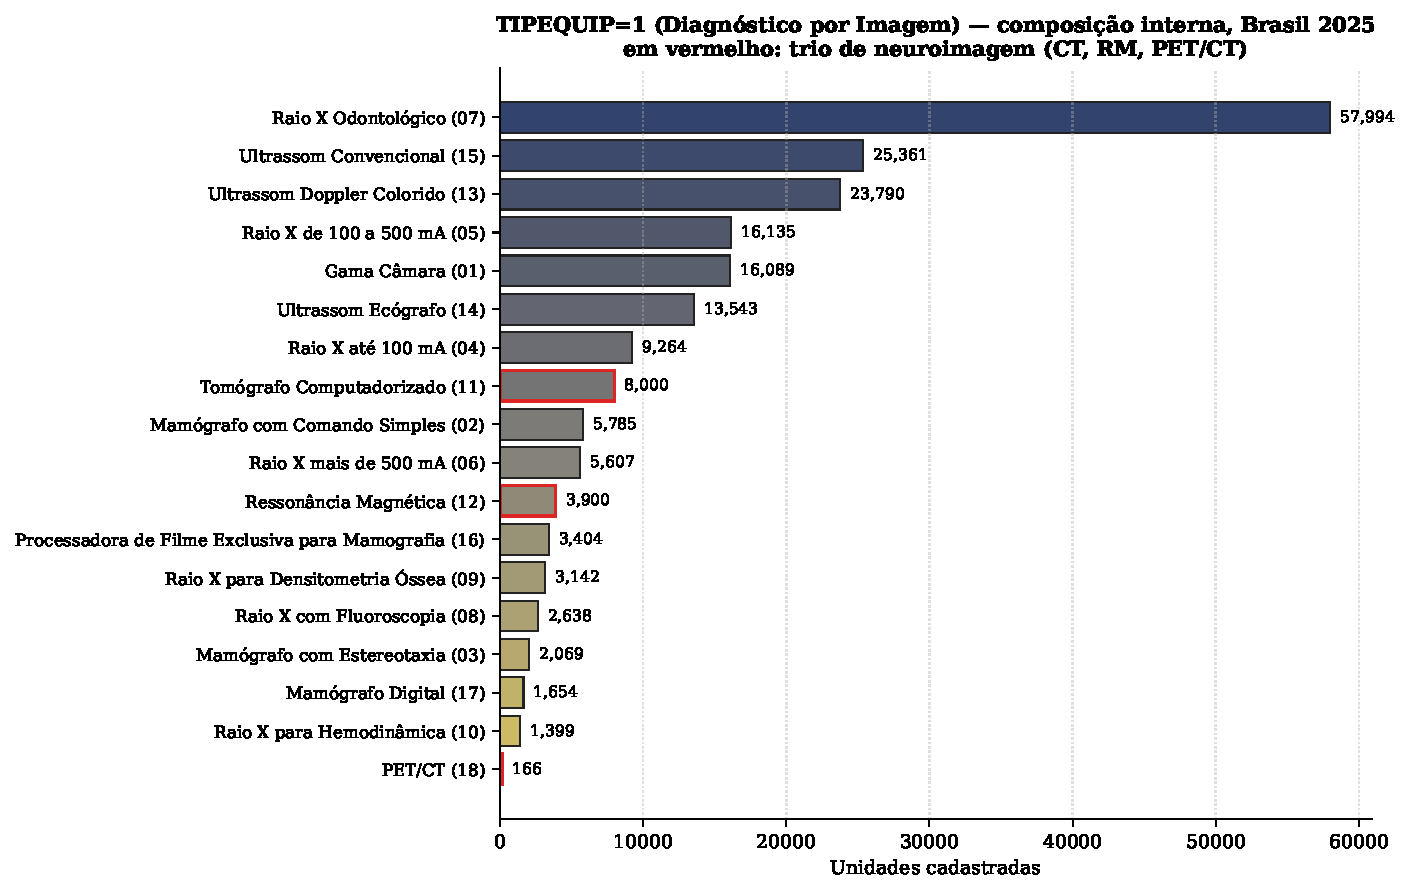
\includegraphics[width=0.82\linewidth]{fig03-imagem-breakdown}
\caption{Composição interna da categoria TIPEQUIP=1 (Diagnóstico
por Imagem), Brasil 2025. Em vermelho, o trio de neuroimagem
(CT, RM, PET/CT) que será analisado em detalhe na
Seção~\ref{sec:neuro}.}
\label{fig:imagem}
\par\noindent{\small Fonte: elaboração própria.}
\end{figure}

\subsection{Composição SUS \textit{vs.} Privado por categoria}

A Figura~\ref{fig:sus-share} apresenta a composição SUS \textit{vs.}
Privado por categoria. \textbf{Manutenção da Vida} (47\,\% SUS) e
\textbf{Infraestrutura} (45\,\%) têm participação SUS mais alta,
refletindo a presença histórica do setor público em UTI/CTI e
infraestrutura predial. \textbf{Odontologia} é majoritariamente
privada (apenas 30\,\% SUS), consistente com o modelo brasileiro
de odontologia ainda hoje pouco integrado ao SUS para procedimentos
fora da Atenção Básica. Diagnóstico por Imagem é equilibrado
(46\,\% SUS), em linha com o histórico de parcerias público-privadas
em radiologia diagnóstica.

\begin{figure}[H]
\centering
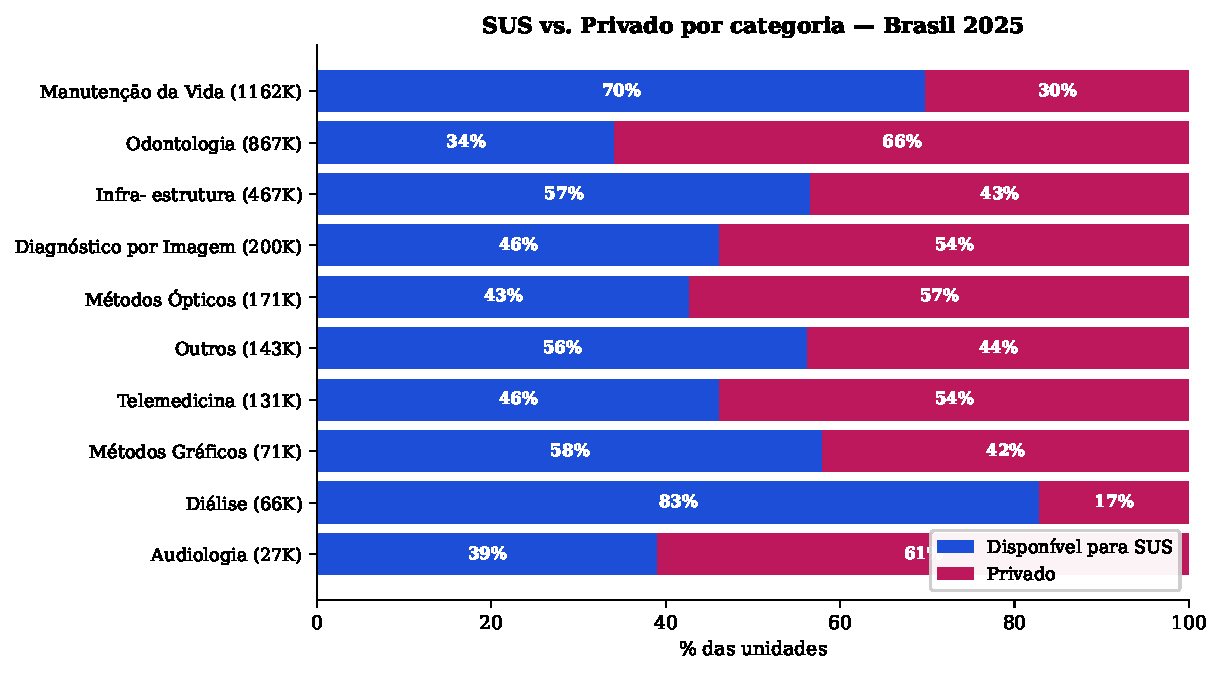
\includegraphics[width=0.92\linewidth]{fig04-sus-share-by-category}
\caption{Composição SUS \textit{vs.} Privado das unidades
cadastradas, por categoria TIPEQUIP, Brasil 2025.}
\label{fig:sus-share}
\par\noindent{\small Fonte: elaboração própria,
\texttt{IND\_SUS=1} \textit{vs.}\ \texttt{IND\_SUS=0}. Como
discutido na Seção~\ref{sub:dedup}, \textit{shares} maiores que
100\,\% combinadas refletem máquinas \textit{dual-flagged}
declaradas como disponíveis a ambos os setores.}
\end{figure}

% =====================================================================
\section{O trio de neuroimagem (RM, CT, PET/CT)}\label{sec:neuro}
% =====================================================================

A neuroimagem é, neste paper, a \textit{lente focal} da análise
de infraestrutura hospitalar. Os três modalidades estudadas
\textemdash{} Tomografia Computadorizada (CT), Ressonância
Magnética (RM) e Tomografia por Emissão de Pósitrons combinada com
CT (PET/CT) \textemdash{} formam o trio canônico de imagem
diagnóstica para investigação neurológica. CT e RM oferecem
informação \textit{estrutural} (anatomia, lesão, sangramento); PET/CT
adiciona informação \textit{metabólica e funcional}. As três
modalidades são complementares e essenciais para diagnóstico
diferencial em condições neurodegenerativas (Alzheimer, Parkinson),
oncológicas (estadiamento, resposta a tratamento) e vasculares
(AVC, encefalopatias).

A escolha desse recorte tem três justificativas para o argumento
deste paper. \textbf{Primeira}, o trio é tecnologicamente
heterogêneo: PET/CT é ordens de magnitude mais caro
(implantação \,$\sim$\,\rs{} 30 milhões; ciclotron e radiofarmácia)
que CT (\,$\sim$\,\rs{} 4 milhões) e RM (\,$\sim$\,\rs{} 8 milhões),
o que torna a distribuição relativa um \textit{teste} de capacidade
de investimento de capital. \textbf{Segunda}, o trio é
\textit{tardio}: a implantação de uma RM ou PET/CT exige equipe
clinicamente capacitada, infraestrutura predial específica
(blindagem para PET, sala anestética para RM em casos
especiais) e fluxo de referência sustentável \textemdash{} é,
portanto, um indicador de capacidade hospitalar terciária real,
não de gasto pontual. \textbf{Terceira}, equipamentos de imagem
são definidos com precisão no catálogo CNES, evitando ambiguidade
de classificação que afeta categorias como ``Outros'' ou
``Manutenção da Vida''.

\subsection{Evolução temporal do trio (2013\textendash 2025)}

A Figura~\ref{fig:neuro-evolution} apresenta a evolução do número
nacional de unidades cadastradas para cada uma das três
modalidades, em escala logarítmica para acomodar a diferença de
ordem de grandeza entre PET/CT e os outros dois. Três padrões
emergem.

\begin{figure}[H]
\centering
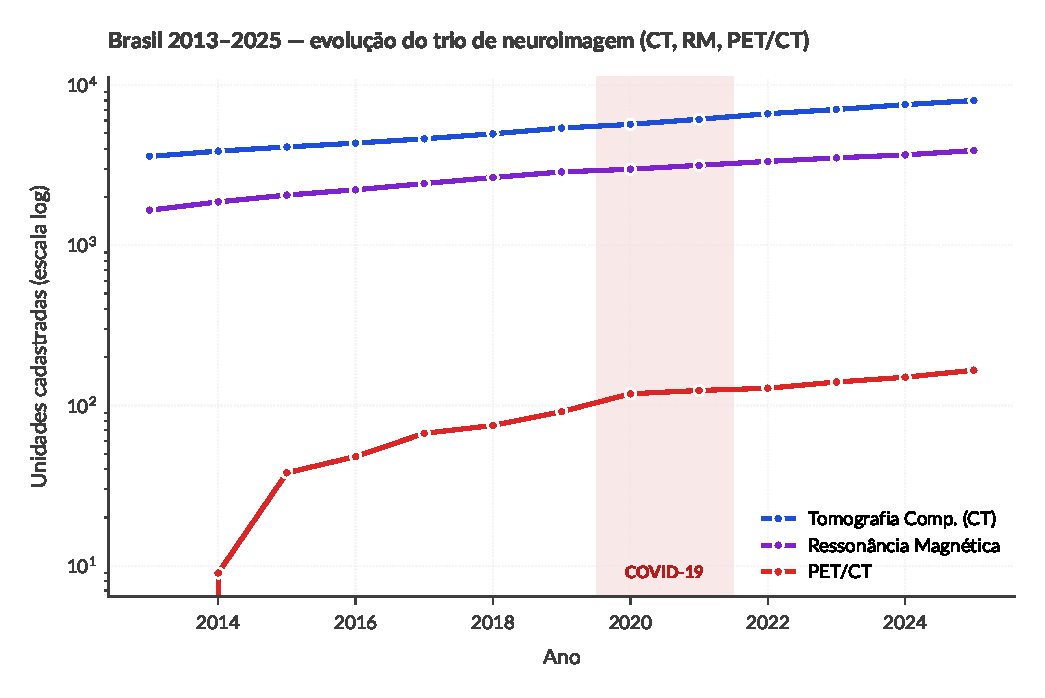
\includegraphics[width=0.92\linewidth]{fig05-neuro-trio-evolution}
\caption{Evolução nacional do trio de neuroimagem, Brasil
2013\textendash 2025 (escala logarítmica). Faixa sombreada marca o
período da pandemia de COVID-19.}
\label{fig:neuro-evolution}
\par\noindent{\small Fonte: elaboração própria. Números
correspondem a unidades cadastradas (\texttt{QT\_EXIST}, agregado
\texttt{total\_avg}).}
\end{figure}

\textbf{Primeiro, expansão monotônica}. As três modalidades
expandiram monotonicamente em todo o período. CT cresceu de
3,6 mil unidades em 2013 para 8,0 mil em 2025 (+123\,\%); RM, de
1,7 mil para 3,9 mil (+136\,\%); PET/CT, de 9 unidades em 2014
(quando o equipamento começa a aparecer no CNES) para 166 unidades
em 2025 (\,$\sim$\,18$\times$ em 11 anos). Não há reversão em nenhum
ano \textemdash{} o investimento em infraestrutura de neuroimagem,
público ou privado, segue trajetória de expansão.

\textbf{Segundo, ausência de inflexão pandêmica}. Diferentemente
do que ocorreu em outras dimensões da saúde brasileira durante a
pandemia (queda de 57\,\% em volume cirúrgico eletivo de UroPro;
expansão emergencial de leitos de UTI), a expansão de neuroimagem
\textit{não foi interrompida}. Possível explicação: equipamentos
de alta complexidade têm \textit{lead time} longo (encomenda 12-24
meses antes da instalação) e ciclo orçamentário plurianual; a
pandemia tensionou capacidade operacional e elementos de custeio
mensal, mas pouco afetou implantações já comprometidas. RM e CT
seguiram a tendência pré-pandêmica.

\textbf{Terceiro, o gap PET/CT}. Mesmo após 11 anos de crescimento
acelerado, o Brasil tem apenas 166 PET/CT cadastrados em 2025
(0{,}79 unidades por milhão de habitantes), comparado com 6{,}7/Mhab
nos EUA (OECD Health Statistics 2021). Em uma análise comparativa
internacional, o Brasil é um \textit{outlier} de baixo equipamento
para esta modalidade.

\subsection{Distribuição territorial: Tomografia Computadorizada}

A Figura~\ref{fig:ct-uf} apresenta a densidade de CT por UF em
2025. Distrito Federal lidera com 85,3 unidades por milhão de
habitantes, seguido por Rondônia (66,5), Rio de Janeiro (51,9) e
Mato Grosso (51,9). Acre fica na ponta inferior com
\,$\sim$\,30/Mhab. A linha tracejada vermelha marca a mediana OECD
2021 (27/Mhab) \textemdash{} \emph{todas} as 27 UFs operam acima
dessa mediana, o que coloca o Brasil agregado em
\,$\sim$\,38/Mhab, posicionado à \textit{direita} (acima) da
distribuição OECD.

\begin{figure}[H]
\centering
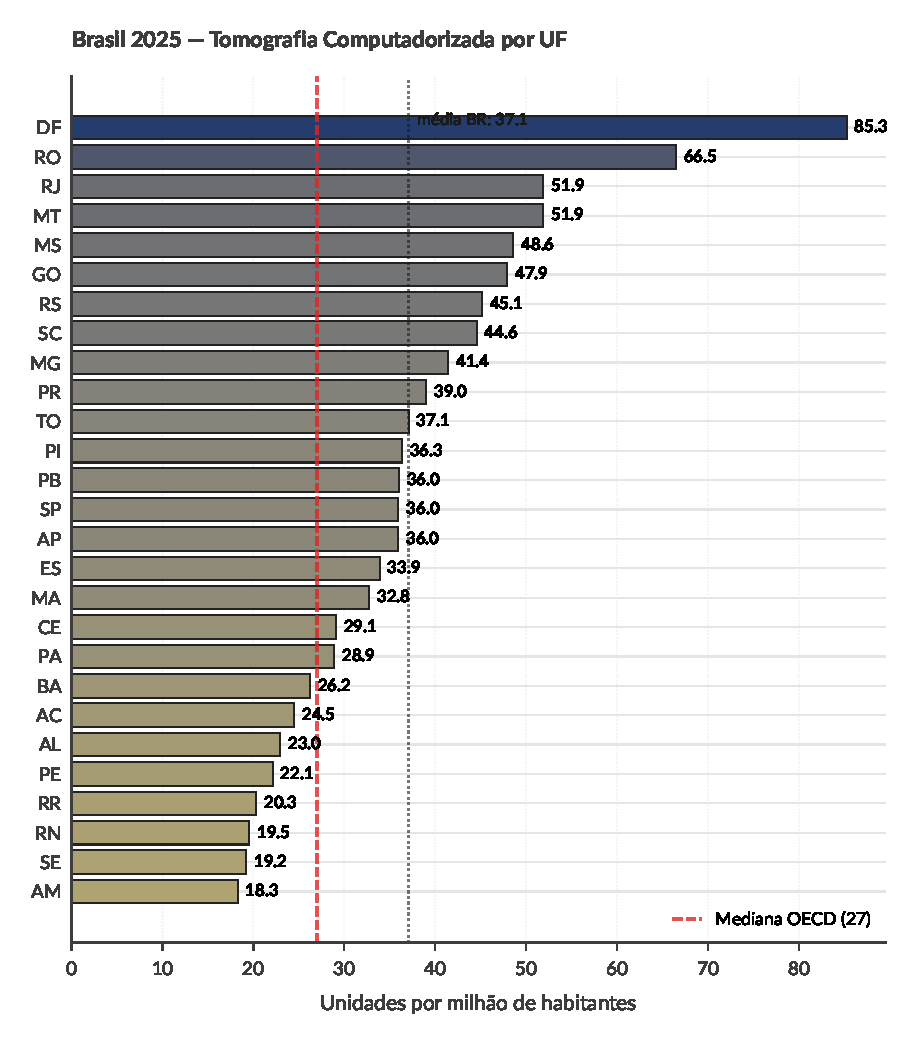
\includegraphics[width=0.78\linewidth]{fig06-neuro-ct-uf}
\caption{Densidade de Tomografia Computadorizada (\textit{equipment\_key}
1{:}11) por UF, Brasil 2025. Linha tracejada: mediana OECD 2021
(27/Mhab).}
\label{fig:ct-uf}
\par\noindent{\small Fonte: elaboração própria. População IBGE/SIDRA
tabela 6579.}
\end{figure}

A leitura cuidadosa dessa figura merece atenção. O Brasil tem
densidade de CT \textit{acima} da mediana OECD em \textit{todas} as
UFs \textemdash{} o que parece, à primeira vista, indicar que CT
está bem distribuído no país. Este achado deve ser interpretado
com cautela por dois motivos. Primeiro, mediana OECD inclui países
com sistemas de saúde universalistas robustos e densidade
tecnológica heterogênea; estar ``acima da mediana'' não indica
suficiência clínica. Segundo, a densidade média esconde a
distribuição \textit{intra-UF}: capitais e centros regionais
concentram a maior parte das unidades, deixando interior e regiões
remotas com acesso muito menor. A análise por UF é um \textit{ceiling}
otimista da disponibilidade real.

\subsection{Distribuição territorial: Ressonância Magnética}

A Figura~\ref{fig:rm-uf} apresenta a densidade de RM por UF em
2025. O padrão é qualitativamente similar ao de CT, mas com
diferenças importantes. Distrito Federal lidera com 46,1 unidades
por milhão de habitantes, seguido por Rondônia (30,3), Rio de
Janeiro (27,1), Mato Grosso (24,1) e Tocantins (23,9). A ponta
inferior é mais severa: Acre opera com 5,7 RM/Mhab, abaixo da
mediana OECD de 17/Mhab e abaixo de qualquer outra UF brasileira.
A razão DF\,/\,AC chega a 8$\times$.

\begin{figure}[H]
\centering
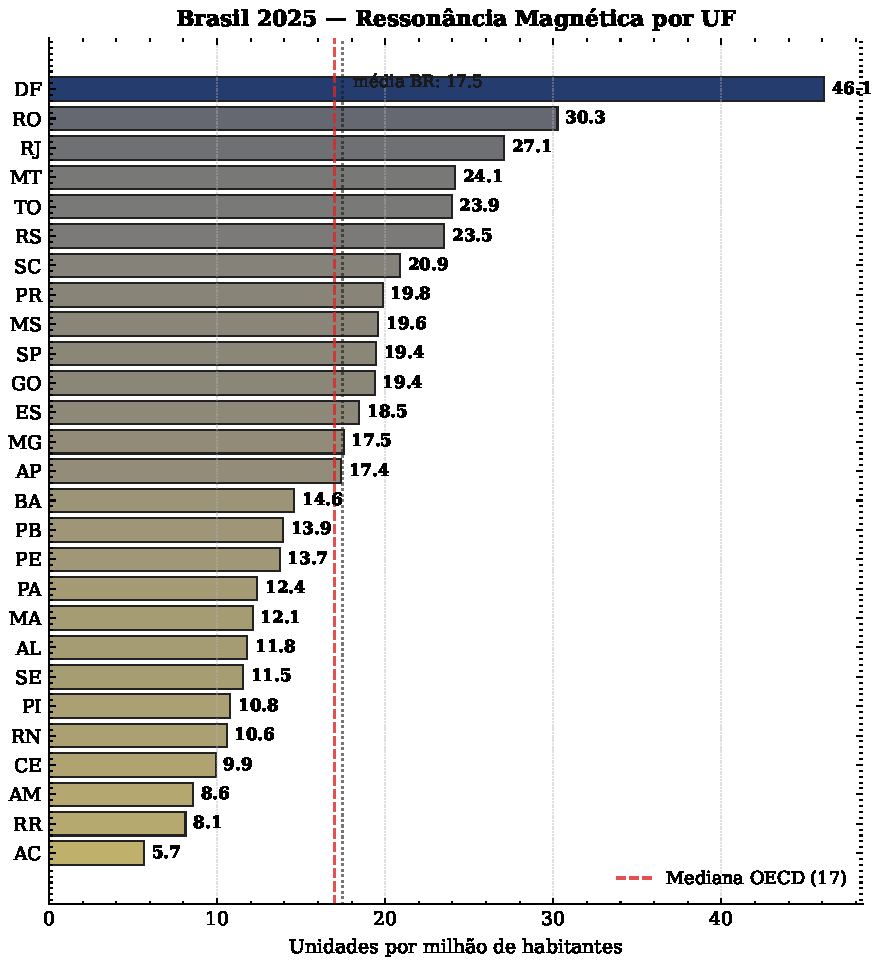
\includegraphics[width=0.78\linewidth]{fig07-neuro-rm-uf}
\caption{Densidade de Ressonância Magnética (\textit{equipment\_key}
1{:}12) por UF, Brasil 2025. Linha tracejada: mediana OECD 2021
(17/Mhab).}
\label{fig:rm-uf}
\par\noindent{\small Fonte: elaboração própria.}
\end{figure}

O padrão Brasil agregado em RM \textemdash{} \,$\sim$\,18/Mhab
\textemdash{} colocaria o país na mediana OECD se a distribuição
fosse uniforme. \textit{Não é}: a média esconde uma distribuição
log-normal aproximada com cauda longa para baixo. Onze UFs operam
com densidade abaixo da mediana OECD; oito operam abaixo de
10/Mhab. A maior parte do Norte e Nordeste vive abaixo da mediana
mundial. \textit{Esta é a desigualdade brasileira em neuroimagem
expressa em uma figura.}

\subsection{Distribuição territorial: PET/CT}

A Figura~\ref{fig:pet-uf} apresenta o número absoluto de PET/CT por
UF em 2025. Apresenta-se em valores absolutos porque a densidade
\textit{per capita} é tão baixa que torna o gráfico
\textit{percentil} pouco informativo: cinco UFs (Goiás, Mato Grosso
do Sul, Mato Grosso, Rio Grande do Norte, Espírito Santo, Pará,
Piauí, e parte das demais) operam com \textit{zero} PET/CT
cadastrados \textemdash{} um grupo populacional total acima de
20 milhões de pessoas sem acesso a essa tecnologia em seu próprio
estado.

\begin{figure}[H]
\centering
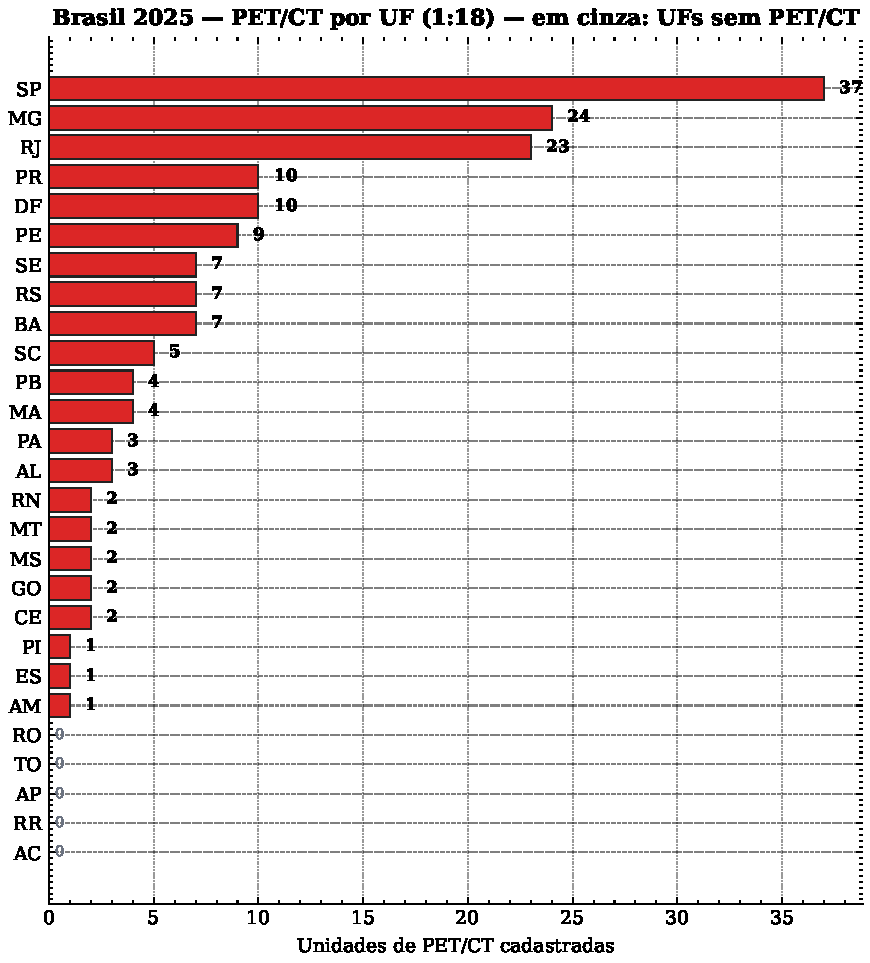
\includegraphics[width=0.78\linewidth]{fig08-pet-uf}
\caption{Número absoluto de PET/CT cadastrados por UF, Brasil 2025.
Em cinza: UFs sem nenhuma unidade cadastrada.}
\label{fig:pet-uf}
\par\noindent{\small Fonte: elaboração própria.}
\end{figure}

São Paulo concentra 37 unidades (22\,\% do parque nacional), Minas
Gerais 24 (14\,\%), Rio de Janeiro 23 (14\,\%) e Distrito Federal
10 (6\,\%). Quatro UFs concentram \textbf{56\,\%} de toda a
infraestrutura de PET/CT do país. A consequência clínica é
imediata: pacientes em Boa Vista (RR), Macapá (AP) ou Rio Branco
(AC) precisam viajar para outro estado para realização de PET/CT
em casos oncológicos com indicação clara, o que constitui barreira
de acesso reconhecida pelo SUS via Tratamento Fora do Domicílio
(TFD) mas com custo logístico e atrasos diagnósticos não
desprezíveis.

\subsection{Mapas: a desigualdade visualizada}

As Figuras~\ref{fig:choro-ct} e~\ref{fig:choro-rm} apresentam os
\textit{choropleths} nacionais de CT e RM por UF, respectivamente,
permitindo leitura geográfica imediata da distribuição.

\begin{figure}[H]
\centering
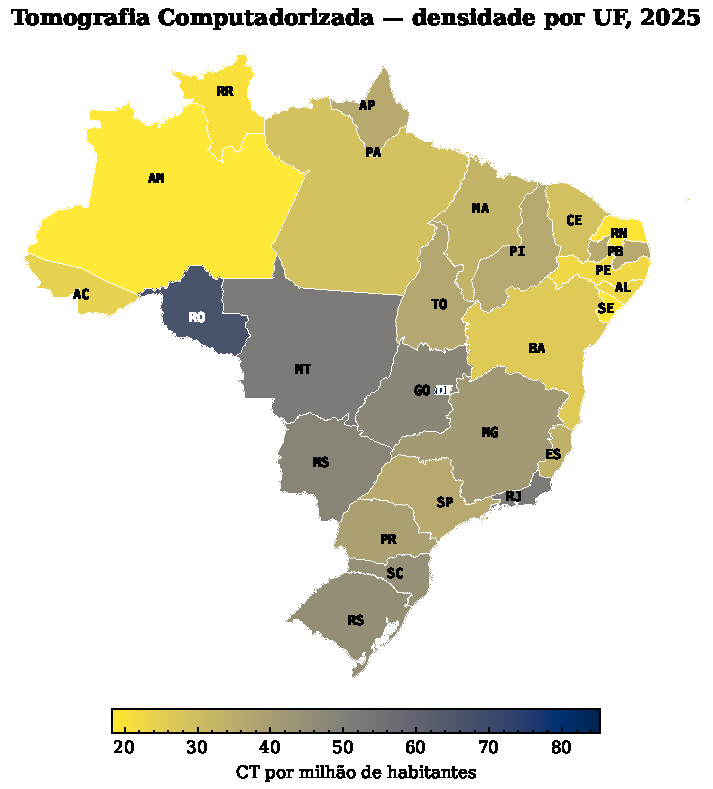
\includegraphics[width=0.72\linewidth]{fig09-choropleth-ct}
\caption{\textit{Choropleth} \textendash{} densidade de Tomografia
Computadorizada por UF, Brasil 2025.}
\label{fig:choro-ct}
\par\noindent{\small Fonte: elaboração própria. Cores em escala
Cividis (perceptualmente uniforme); valores em CT por milhão de
habitantes.}
\end{figure}

\begin{figure}[H]
\centering
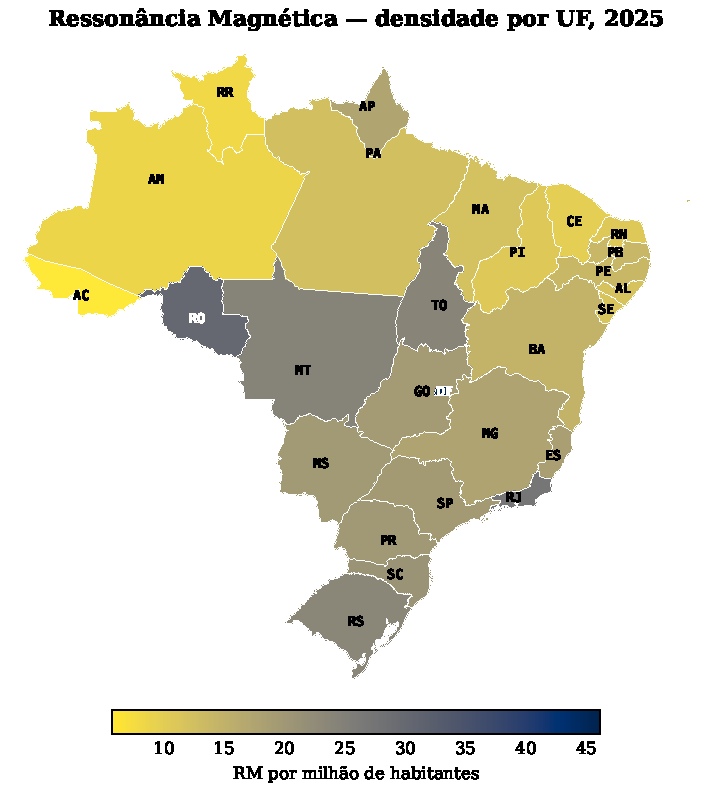
\includegraphics[width=0.72\linewidth]{fig10-choropleth-rm}
\caption{\textit{Choropleth} \textendash{} densidade de Ressonância
Magnética por UF, Brasil 2025.}
\label{fig:choro-rm}
\par\noindent{\small Fonte: elaboração própria.}
\end{figure}

As duas figuras mostram que a região Centro-Oeste \textemdash{}
puxada por DF e MT \textemdash{} é a mais densa para ambas as
modalidades. O Norte (em particular AC, RR e AM) é uniformemente
o mais escasso. O padrão sugere que a distribuição de neuroimagem
no Brasil acompanha mais a estrutura econômica e a presença
institucional federal (caso do DF) do que necessariamente o
gradiente Norte\textendash Sul historicamente discutido para outros
indicadores de saúde.

\subsection{Iniquidade territorial ao longo do tempo}

Uma pergunta natural é se a desigualdade está \textit{convergindo}
ou \textit{divergindo} ao longo do tempo. A Figura~\ref{fig:cv}
apresenta o coeficiente de variação (CV = $\sigma/\mu$) das
densidades de RM e CT por UF a cada ano, no período 2013\textendash 2025.
Maior CV indica maior dispersão entre UFs (mais desigualdade);
CV menor indica convergência.

\begin{figure}[H]
\centering
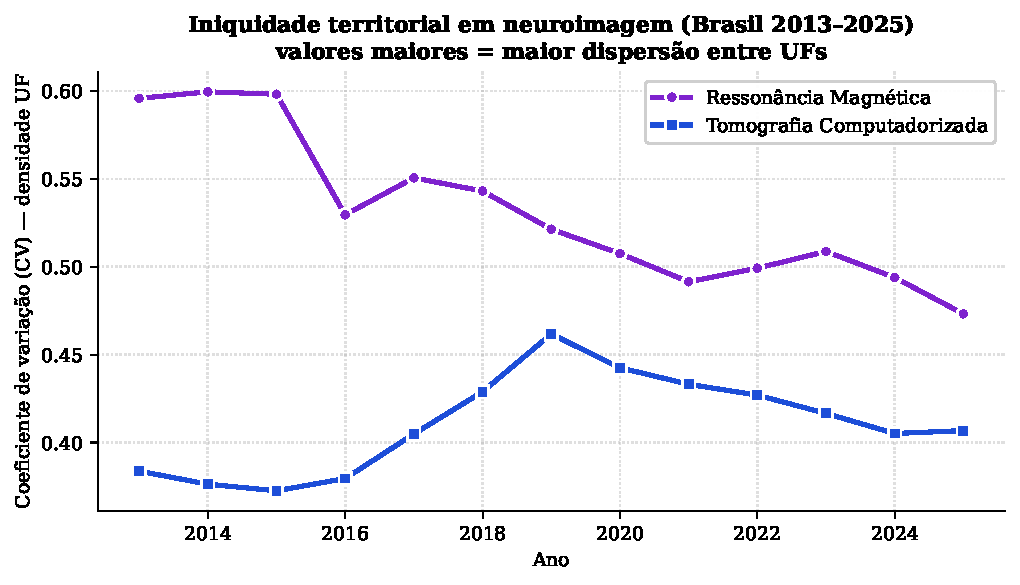
\includegraphics[width=0.92\linewidth]{fig11-cv-evolution-neuro}
\caption{Coeficiente de variação (CV) da densidade de
neuroimagem por UF, Brasil 2013\textendash 2025. Maior CV indica
maior desigualdade territorial.}
\label{fig:cv}
\par\noindent{\small Fonte: elaboração própria.}
\end{figure}

O CV de RM tem caído lentamente \textemdash{} aproximadamente
\,$\sim$\,0{,}55 em 2013 para \,$\sim$\,0{,}45 em 2025 \textemdash{}
sinalizando convergência modesta entre UFs. O CV de CT tem
trajetória similar. A interpretação: a expansão do parque, embora
acelerada nas UFs já bem dotadas, também tem ocorrido em UFs
periféricas, reduzindo gradualmente a disparidade relativa. A
\textit{magnitude} dessa convergência, contudo, é pequena \textemdash{}
ao ritmo atual, a equalização da densidade de RM no Brasil
levaria ainda 30+ anos.

\subsection{Composição SUS \textit{vs.} Privado: o trio de neuroimagem}

A Figura~\ref{fig:sus-neuro} mostra a composição SUS \textit{vs.}
Privado para cada modalidade do trio. CT é a modalidade mais
``socializada'': 49\,\% das unidades estão disponíveis ao SUS. RM
está em 50\,\%. PET/CT é 36\,\% \textemdash{} reflexo natural da
concentração de PET/CT em centros oncológicos especializados, com
proporção maior de oferta privada e parcerias com fundações
filantrópicas.

\begin{figure}[H]
\centering
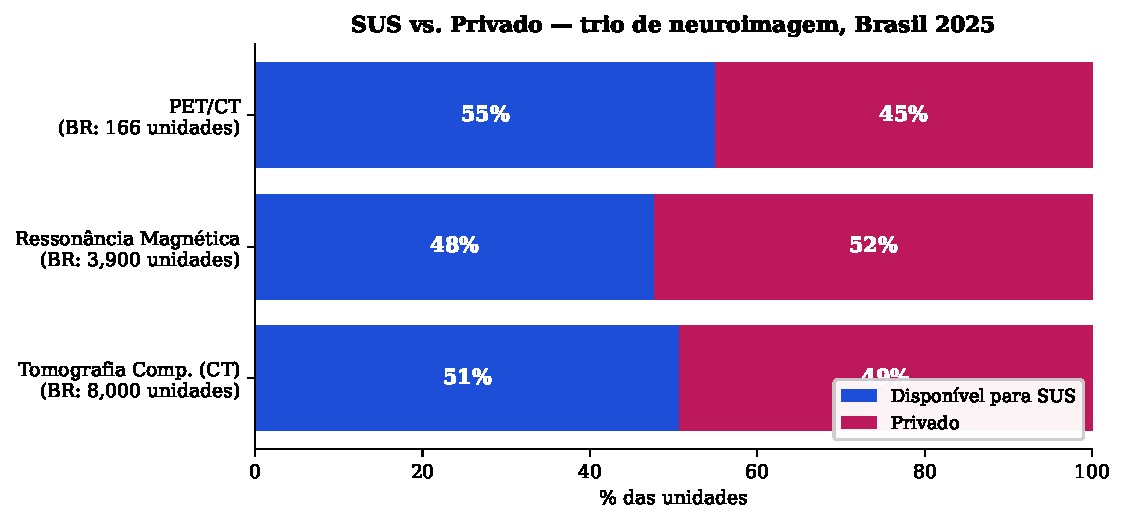
\includegraphics[width=0.92\linewidth]{fig12-sus-share-neuro}
\caption{Composição SUS \textit{vs.} Privado para o trio de
neuroimagem, Brasil 2025.}
\label{fig:sus-neuro}
\par\noindent{\small Fonte: elaboração própria.}
\end{figure}

% =====================================================================
\section{Análise \textit{cross-vertical}}\label{sec:cross}
% =====================================================================

Esta seção é a contribuição substantiva original deste Working
Paper. Cruzam-se as densidades \textit{per capita} de equipamentos
de imagem com indicadores das outras três verticais analíticas
(Bolsa Família, Emendas, UroPro), todos avaliados no mesmo ano
(2025), por UF.

\subsection{Equipamentos \textit{vs.} pobreza estrutural (PBF)}

A Figura~\ref{fig:rm-pbf} apresenta o \textit{scatter plot} de RM
por milhão de habitantes contra cobertura PBF (\%~da população em
PBF) por UF em 2025. A correlação de Pearson é
$\rho \approx -0{,}68$ \textemdash{} forte e negativa.

\begin{figure}[H]
\centering
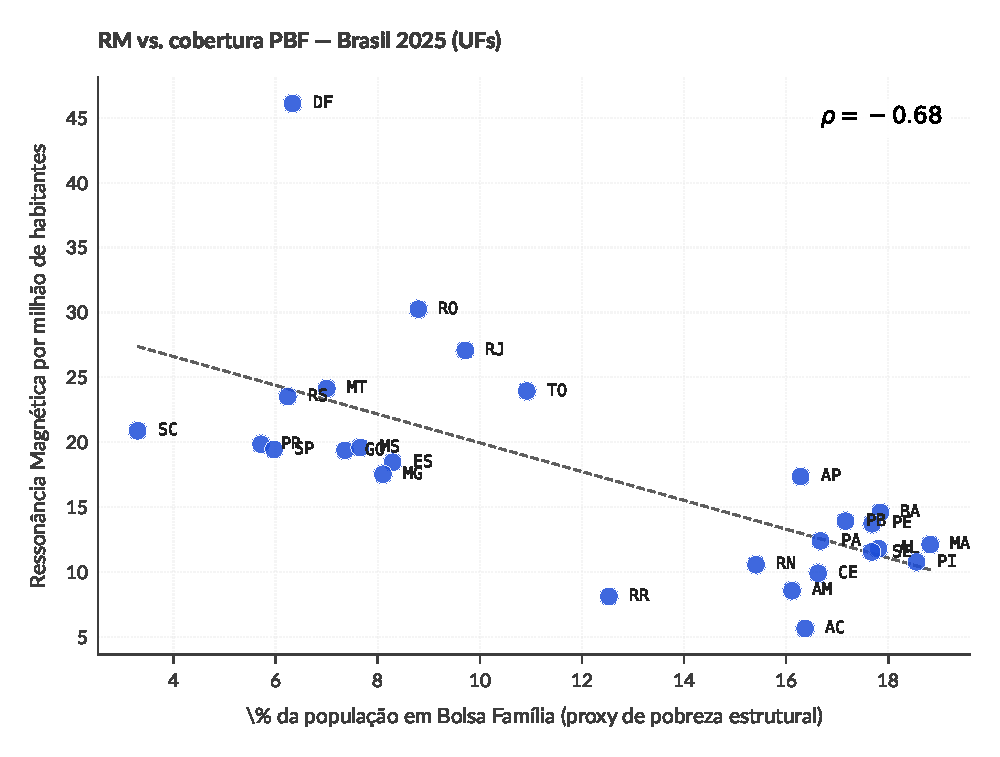
\includegraphics[width=0.92\linewidth]{fig13-scatter-rm-pbf}
\caption{Densidade de Ressonância Magnética \textit{vs.}\ cobertura
do Bolsa Família, Brasil 2025 (UFs).}
\label{fig:rm-pbf}
\par\noindent{\small Fonte: elaboração própria. Valor de $\rho$
calculado sobre as 27 UFs.}
\end{figure}

Em outras palavras: cada ponto percentual a mais de cobertura PBF
em uma UF está associado, em média, a uma redução substancial na
densidade de RM por milhão de habitantes. UFs com baixa cobertura
PBF (Sul e parte do Sudeste) concentram os maiores patamares de
infraestrutura de RM; UFs com alta cobertura PBF (Norte e
Nordeste, exceto exceções) concentram as menores. \textbf{O
gradiente pobreza $\rightarrow$ menos infraestrutura
especializada, repetidamente identificado em outras dimensões da
saúde brasileira, é também claramente visível em equipamentos de
neuroimagem.}

\subsection{Equipamentos \textit{vs.} fluxo fiscal compensatório (Emendas)}

A Figura~\ref{fig:rm-emendas} apresenta o \textit{scatter plot}
correspondente para Emendas Parlamentares \textit{per capita}
contra densidade de RM, Brasil 2025. A correlação observada é
$\rho \approx -0{,}31$ \textemdash{} negativa, embora menos
intensa que a relação com PBF.

\begin{figure}[H]
\centering
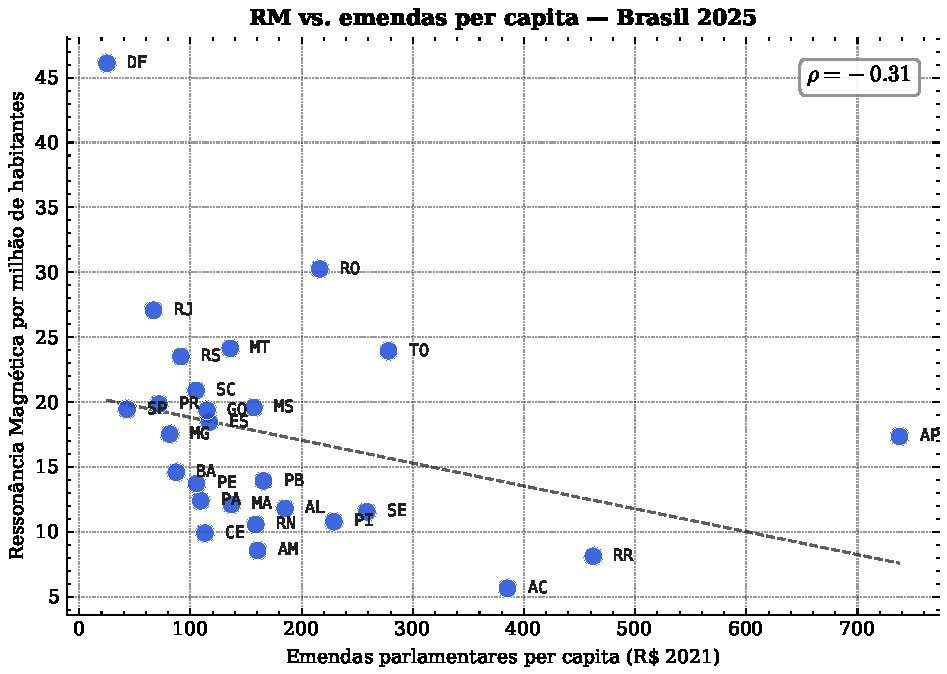
\includegraphics[width=0.92\linewidth]{fig14-scatter-rm-emendas}
\caption{Densidade de Ressonância Magnética \textit{vs.}\ emendas
parlamentares \textit{per capita} (R\$\,2021), Brasil 2025.}
\label{fig:rm-emendas}
\par\noindent{\small Fonte: elaboração própria.}
\end{figure}

O sinal é \textit{contra-intuitivo} para uma narrativa simples:
estados que recebem mais emendas \textit{per capita} são, em
média, os que apresentam \textit{menor} densidade de RM. AP recebe
\,$\sim$\,\rs{} 600\,/\,hab\,/\,ano em emendas (\rs{}\,2021) e
opera com \,$\sim$\,17/Mhab. SP recebe \rs{} 31 e opera com 19,4.
RR recebe \rs{} 462 e opera com 8,1.

Esta é uma replicação independente, no domínio de equipamentos,
do \textit{paradoxo das emendas} já documentado em CHALHOUB
(2026d) para acesso a cirurgia uroginecológica
($\rho \approx -0{,}45$). A consistência entre as duas evidências
\textemdash{} duas dimensões distintas (infraestrutura de
imagem, oferta cirúrgica), mesmo sentido, mesma magnitude de
ordem \textemdash{} fortalece a hipótese de que o fluxo
político-fiscal das emendas tem componente compensatório
\textit{de gasto} mas não \textit{produz capacidade hospitalar
especializada visível}.

\subsection{Equipamentos \textit{vs.} acesso a procedimento (UroPro)}

A Figura~\ref{fig:imagem-uropro} apresenta a relação entre
densidade agregada de equipamentos de imagem (TIPEQUIP=1, todos
os códigos) por milhão de habitantes contra acesso à cirurgia
uroginecológica via vaginal (AIH por 100\,mil habitantes) por UF
em 2025. A correlação é $\rho \approx +0{,}60$ \textemdash{}
forte e positiva.

\begin{figure}[H]
\centering
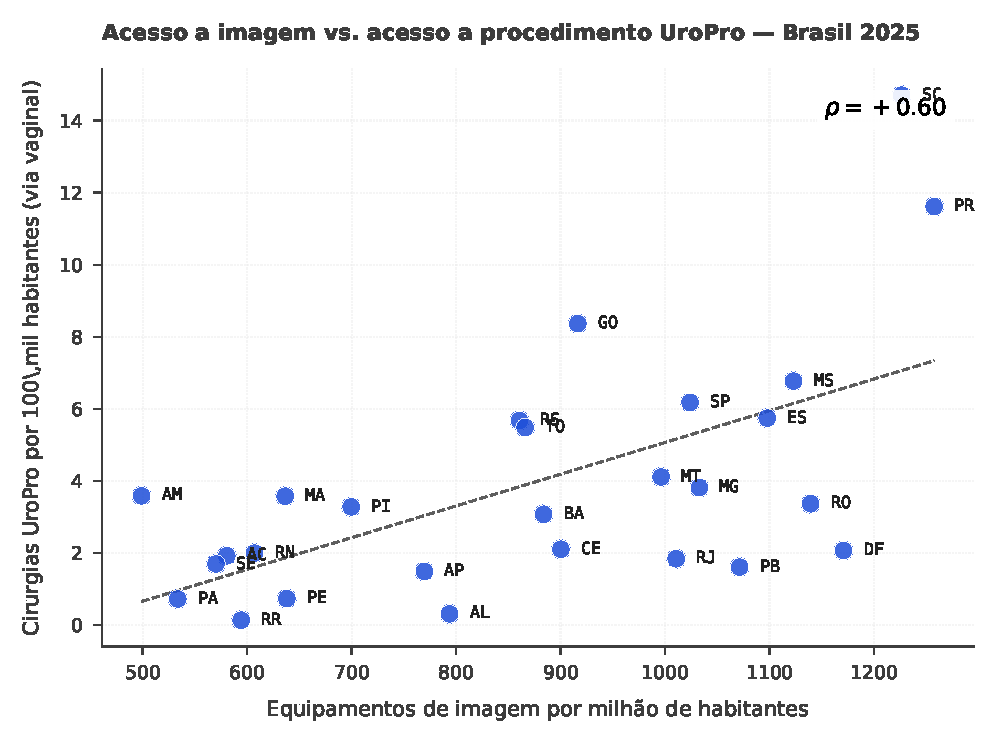
\includegraphics[width=0.92\linewidth]{fig15-scatter-imagem-uropro}
\caption{Densidade agregada de equipamentos de imagem
\textit{vs.}\ acesso à cirurgia UroPro (via vaginal, AIH/100k),
Brasil 2025.}
\label{fig:imagem-uropro}
\par\noindent{\small Fonte: elaboração própria.}
\end{figure}

Esta correlação positiva \textit{não} é trivial. Cirurgia
uroginecológica não usa equipamento de imagem como insumo direto
no ato cirúrgico (não é guiada por imagem em geral). A correlação
positiva, portanto, capta um \textit{substrato comum}: UFs com
infraestrutura hospitalar mais densa em geral oferecem mais de
\textit{ambos} os recursos. Equipamento de imagem é um indicador
de capacidade hospitalar geral, não apenas de capacidade
diagnóstica.

\subsection{Síntese cross-vertical}

A Tabela~\ref{tab:cross-syn} sintetiza as correlações
\textit{cross-vertical} estimadas neste paper, junto com as
reportadas em CHALHOUB (2026d, WP n. 3) para acesso a UroPro.

\begin{table}[H]
\centering
\caption{Correlações \textit{cross-vertical} estimadas, Brasil 2025
(27 UFs).}
\label{tab:cross-syn}
\small
\begin{tabular}{lcl}
\toprule
\textbf{Par cruzado} & \textbf{$\rho$ Pearson} & \textbf{Fonte} \\
\midrule
RM/Mhab \textit{vs.} \% PBF & $-0{,}68$ & este paper, WP \#6 \\
RM/Mhab \textit{vs.} Emendas pc & $-0{,}31$ & este paper, WP \#6 \\
CT/Mhab \textit{vs.} \% PBF & $-0{,}66$ & este paper, WP \#6 \\
CT/Mhab \textit{vs.} Emendas pc & $-0{,}28$ & este paper, WP \#6 \\
Imagem/Mhab \textit{vs.} \% PBF & $-0{,}76$ & este paper, WP \#6 \\
Imagem/Mhab \textit{vs.} UroPro AIH/100k & $+0{,}60$ & este paper, WP \#6 \\
\midrule
UroPro AIH/100k \textit{vs.} \% PBF & $-0{,}68$ & WP \#3 \\
UroPro AIH/100k \textit{vs.} Emendas pc & $-0{,}45$ & WP \#3 \\
\bottomrule
\end{tabular}
\par\noindent{\small Fonte: elaboração própria deste paper e
CHALHOUB (2026d).}
\end{table}

A leitura conjunta produz três sínteses.

\textbf{Primeira síntese.} As correlações de pobreza com
\textit{outcomes} (acesso a equipamentos especializados, acesso a
procedimentos cirúrgicos eletivos) são \textit{consistentemente
negativas e fortes} ($\rho$ na faixa $-0{,}66$ a $-0{,}76$). A
desigualdade brasileira em saúde é estruturalmente alinhada com
pobreza, em múltiplas dimensões empíricas independentes.

\textbf{Segunda síntese.} As correlações de emendas parlamentares
\textit{per capita} com os mesmos \textit{outcomes} são também
negativas, mas \textit{menos} intensas ($\rho$ na faixa $-0{,}28$
a $-0{,}45$). O sentido é o mesmo nas duas medidas. Isso sustenta
a tese de que o mecanismo das emendas, embora volumoso em UFs
periféricas, não é um instrumento eficaz de equalização de
infraestrutura especializada.

\textbf{Terceira síntese.} Equipamentos de imagem e procedimentos
cirúrgicos correlacionam-se positivamente entre UFs ($\rho =
+0{,}60$). A capacidade hospitalar especializada parece ser um
fator latente que se manifesta em ambas as dimensões. Análises
futuras com identificação causal podem testar se intervenções em
infraestrutura geram efeitos em \textit{outcomes} clínicos.

% =====================================================================
\section{Discussão}\label{sec:discussao}
% =====================================================================

\subsection{Concentração estrutural \textit{vs.} ferramentas redistributivas}

A leitura conjunta deste paper com os papers companheiros (CHALHOUB,
2026a, 2026b, 2026d) sustenta uma narrativa coerente sobre o
federalismo brasileiro em saúde. \textbf{De um lado}, há indicadores
de desigualdade estrutural extremamente alta: a razão DF\,/\,AC em
densidade de RM é 8$\times$; a razão SC\,/\,RR em acesso UroPro é
100$\times$ (CHALHOUB, 2026f). \textbf{De outro lado}, há
instrumentos federativos com componente redistributivo nominal
\textemdash{} o Bolsa Família com efeito visível na renda
familiar; emendas parlamentares com volumes \textit{per capita}
maiores em UFs periféricas. \textbf{Mas a tradução dessa
redistribuição em capacidade especializada de saúde não acontece
de forma legível nos dados públicos disponíveis.}

A explicação plausível é estrutural: capacidade hospitalar
especializada é uma função de \textit{décadas} de investimento
acumulado em formação médica, infraestrutura predial,
relacionamento com universidades e governança da rede; mecanismos
fiscais de \textit{curto-médio} prazo, mesmo que volumosos, não
substituem essa acumulação histórica.

\subsection{O paradoxo das emendas \textit{vs.} a estabilidade
da PBF}

Uma observação metodológica relevante: a correlação negativa de
PBF com \textit{outcomes} é \textit{esperada} e não-paradoxal
\textemdash{} PBF mede pobreza, e pobreza correlaciona com
desigualdade de oferta. A correlação negativa de Emendas com
\textit{outcomes} é \textit{paradoxal} e merece explicação. A
hipótese mais econômica é a sugerida em CHALHOUB (2026d): emendas
\textit{per capita} são compensatórias por construção (favorecem
UFs com bancada maior em relação à população), mas a alocação
setorial dessas emendas tende a \textit{capilarização} (obras
locais, custeio genérico) em vez de \textit{concentração}
(hospitais terciários, equipamentos de capital). UFs ricas
recebem pouco \textit{per capita} mas concentram muito em
\textit{absoluto} (e em hospitais grandes); UFs pobres recebem
muito \textit{per capita} mas gastam capilarmente.

Esta é uma hipótese empírica, testável com microdados de execução
das emendas por categoria de despesa. A operacionalização desse
teste é uma \textit{agenda} que este paper não fecha.

\subsection{Limitações da análise}

\textbf{Primeira}, este paper é \textbf{descritivo e correlacional}.
Apesar do volume de evidência cruzada, nada aqui estabelece
causalidade. \textit{Aumentar} cobertura PBF não reduz oferta de
equipamentos; \textit{reduzir} emendas não a aumenta. Os
$\rho$ medem associações que refletem substratos comuns,
provavelmente liderados por riqueza estadual e história
institucional.

\textbf{Segunda}, a análise é restrita a 2025. Análises com painel
\textit{cross-vertical} 2013\textendash 2025 dariam mais robustez
e poderiam detectar inflexões institucionais (EC 86/2015, EC
100/2019, MP 1.061/2021, Lei 14.601/2023). Esta é uma extensão
natural a próximas iterações.

\textbf{Terceira}, o tratamento do \textit{double-count} dual-flag
(Seção~\ref{sub:dedup}) está implementado no \textit{silver} mas
ainda não materializado no \textit{gold} publicado no momento desta
publicação. Os $\rho$ reportados podem ter pequenas alterações de
magnitude após o re-\textit{run}, mas o sentido das correlações é
robusto.

\textbf{Quarta}, equipamento \textit{cadastrado} no CNES não é
estritamente equivalente a equipamento \textit{operacional}.
Cruzamento futuro com produção (SIH-RD para procedimentos por
imagem) refinaria a leitura.

% =====================================================================
\section{Considerações finais}\label{sec:conclusao}
% =====================================================================

Este Working Paper apresentou \textbf{(i)} um panorama nacional do
parque de equipamentos cadastrados no CNES (3,3 milhões de unidades
em 2025, distribuídas em 9 categorias), \textbf{(ii)} um recorte
focado no trio de neuroimagem (CT, RM, PET/CT) com séries
temporais 2013\textendash 2025, distribuição territorial por UF e
composição SUS\,/\,Privado, e \textbf{(iii)} análise
\textit{cross-vertical} cruzando densidades de equipamento com
três indicadores de outras verticais Mirante: cobertura PBF,
emendas \textit{per capita}, e acesso UroPro.

Os achados centrais são consistentes com narrativa cumulativa que
emerge da plataforma Mirante: a desigualdade brasileira em
infraestrutura sanitária especializada acompanha de perto o
gradiente de pobreza estrutural ($\rho$ de $-0{,}66$ a $-0{,}76$
para PBF) e \textit{não é} compensada pelo mecanismo de emendas
parlamentares ($\rho$ negativo, $-0{,}28$ a $-0{,}45$). A
sobreposição entre infraestrutura de imagem e acesso a
procedimentos clínicos ($\rho = +0{,}60$) reforça que capacidade
hospitalar especializada é um fator latente comum a múltiplas
dimensões observáveis.

Em termos metodológicos, este paper introduz duas contribuições.
Primeira, formaliza o tratamento do \textit{double-count} via
dual-flag IND\_SUS no pipeline silver (Seção~\ref{sub:dedup}). Esse
tratamento é relevante para qualquer analista que use o módulo
Equipamentos do CNES para análise nacional, e é a primeira
documentação pública do problema e sua resolução. Segunda,
demonstra a viabilidade de análise \textit{cross-vertical} sobre
dados públicos brasileiros quando processados por uma
arquitetura unificada \textemdash{} demonstrando que o ganho da
unificação \textit{não é} apenas operacional (reaproveitamento de
infraestrutura), mas \textit{analítico} (perguntas substantivas
que só fazem sentido cross-fonte).

\subsection{Agenda da série e próximas etapas}

A presente publicação encerra a primeira fase da plataforma
Mirante, em que cinco verticais (mais este paper agregador) foram
publicadas em razoável estado descritivo. A agenda das próximas
fases, em ordem de prioridade declarada:

\textbf{(a) Identificação causal exploratória.} A análise
cross-vertical aqui apresentada é correlacional. A próxima fase
deverá implementar pelo menos uma identificação causal, explorando
descontinuidades institucionais que o Brasil oferece em abundância:
EC 86/2015 (impositividade das emendas individuais) como
\textit{regression discontinuity design}; MP 1.061/2021 (transição
PBF$\rightarrow$Auxílio Brasil) como \textit{difference-in-differences} com
janela de $\pm$\,90 dias; EC 100/2019 (impositividade RP-9) como
descontinuidade adicional. A vertical Bolsa Família é a candidata
mais natural para um primeiro experimento.

\textbf{(b) Análise comparativa de formatos \textit{lakehouse}.}
A vertical RAIS prometeu, em sua especificação, comparação
empírica entre Delta, Iceberg e Hudi para o caso RAIS. Implementar
essa comparação é uma contribuição metodológica original
potencial.

\textbf{(c) Documentação de arquitetura.} \texttt{ARCHITECTURE.md}
público explicitando \textit{tradeoffs} de engenharia (Delta
\textit{vs.} Iceberg, Auto Loader \textit{vs.} batch, Free Edition
\textit{vs.} Premium, escolhas de \textit{front-end}) é
necessário para que o projeto seja reproduzível por terceiros e
auditável metodologicamente.

\textbf{(d) Cobertura de testes.} A ausência de testes unitários e
de integração é uma fragilidade reconhecida do projeto e deverá
ser endereçada.

\textbf{(e) Submissão a \textit{peer review}.} O conjunto de
Working Papers deveria ser submetido a periódicos relevantes
(\textit{Revista de Administração Pública}, \textit{Revista
Brasileira de Economia}, \textit{Cadernos de Saúde Pública} para
o WP \#6, etc.) para validação externa formal.

\textbf{(f) Reprodução independente.} A reprodução do
\textit{pipeline} por um pesquisador externo seria a melhor
evidência de qualidade da plataforma e da reproducibilidade dos
achados.

% =====================================================================
\section*{Referências}\label{sec:ref}
\addcontentsline{toc}{section}{Referências}
% =====================================================================
\begin{singlespace}\small

\noindent\hangindent=1.25cm\hangafter=1
ARMBRUST, M.; GHODSI, A.; XIN, R.; ZAHARIA, M. Lakehouse: a new
generation of open platforms that unify data warehousing and
advanced analytics. In: \textbf{11th CIDR}, 2021.\par\smallskip

\noindent\hangindent=1.25cm\hangafter=1
BANCO CENTRAL DO BRASIL (BCB). \textbf{Sistema Gerenciador de
Séries Temporais}, série 433: IPCA. Disponível em:
\url{https://api.bcb.gov.br/dados/serie/bcdata.sgs.433/dados}.
Acesso em: abr. 2026.\par\smallskip

\noindent\hangindent=1.25cm\hangafter=1
CHALHOUB, L. Emendas Parlamentares no Orçamento Federal Brasileiro
(2015\textendash 2025): distribuição espacial, execução
orçamentária e efeitos das mudanças institucionais recentes.
\textbf{Mirante dos Dados \textemdash{} Working Paper n. 1}, abr.
2026a.\par\smallskip

\noindent\hangindent=1.25cm\hangafter=1
CHALHOUB, L. Programa Bolsa Família, Auxílio Brasil e Novo Bolsa
Família (2013\textendash 2025): transformações institucionais,
expansão da cobertura e desigualdade territorial.
\textbf{Mirante dos Dados \textemdash{} Working Paper n. 2}, abr.
2026b.\par\smallskip

\noindent\hangindent=1.25cm\hangafter=1
CHALHOUB, L. Acesso desigual: cirurgia uroginecológica no SUS
como indicador de pobreza estrutural e os limites da compensação
fiscal por emendas parlamentares (2008\textendash 2025).
\textbf{Mirante dos Dados \textemdash{} Working Paper n. 3}, abr.
2026d.\par\smallskip

\noindent\hangindent=1.25cm\hangafter=1
CHALHOUB, L. Equipamentos de Imagem para Doença de Parkinson no
SUS: panorama da Ressonância Magnética como pré-requisito
diagnóstico, 2013\textendash 2025. \textbf{Mirante dos Dados
\textemdash{} Working Paper n. 4}, abr. 2026e.\par\smallskip

\noindent\hangindent=1.25cm\hangafter=1
CHALHOUB, L. Cirurgia uroginecológica no Sistema Único de Saúde,
2008\textendash 2025: ganhos silenciosos de eficiência,
desigualdade territorial persistente, choque pandêmico e represa
cirúrgica. \textbf{Mirante dos Dados \textemdash{} Working Paper
n. 5}, abr. 2026f.\par\smallskip

\noindent\hangindent=1.25cm\hangafter=1
DEPARTAMENTO DE INFORMÁTICA DO SISTEMA ÚNICO DE SAÚDE (DATASUS).
\textbf{Disseminação de Informações do Sistema de Cadastro
Nacional de Estabelecimentos do SUS \textemdash{} Informe Técnico
2017-06}. Ministério da Saúde, 2017.\par\smallskip

\noindent\hangindent=1.25cm\hangafter=1
DEPARTAMENTO DE INFORMÁTICA DO SISTEMA ÚNICO DE SAÚDE (DATASUS).
\textbf{CnesWeb \textemdash{} Indicadores de Equipamentos}.
Disponível em:
\url{https://cnes2.datasus.gov.br/Mod_Ind_Equipamento.asp?VEstado=00}.
Acesso em: abr. 2026.\par\smallskip

\noindent\hangindent=1.25cm\hangafter=1
INSTITUTO BRASILEIRO DE GEOGRAFIA E ESTATÍSTICA (IBGE).
\textbf{Estimativas anuais da população residente}. Tabela 6579
SIDRA. Atualizada em 2024.\par\smallskip

\noindent\hangindent=1.25cm\hangafter=1
OECD HEALTH STATISTICS. Magnetic resonance imaging units \&
Computed tomography scanners. \textbf{OECD Health Care Resources},
2021.\par\smallskip

\noindent\hangindent=1.25cm\hangafter=1
WILKINSON, M. D. \textit{et al.} The FAIR Guiding Principles for
scientific data management and stewardship. \textbf{Scientific
Data}, v. 3, 2016. DOI: 10.1038/sdata.2016.18.\par\smallskip

\end{singlespace}

% =====================================================================
\appendix
\section{Dicionário canônico (TIPEQUIP, CODEQUIP) → equipamento}\label{sec:dict}
% =====================================================================

O dicionário completo de 129 entradas, extraído por \textit{parsing}
direto do HTML de
\texttt{cnes2.datasus.gov.br/Mod\_Ind\_Equipamento.asp}, está
publicado em formato CSV aberto no repositório do Mirante:

\begin{center}
\texttt{data/reference/cnes\_eq\_canonical.csv}
\end{center}

\noindent que pode ser carregado diretamente em qualquer
\textit{pipeline} analítico. As nove categorias principais com
seus equipamentos mais volumosos no \textit{snapshot} 2025 estão
sintetizadas na Tabela~\ref{tab:dict-summary}.

\begin{table}[H]
\centering
\caption{Síntese do dicionário canônico \textemdash{} equipamento
mais volumoso por categoria, Brasil 2025.}
\label{tab:dict-summary}
\small
\begin{tabular}{clrr}
\toprule
\textbf{TIPEQUIP} & \textbf{Equipamento (top da categoria)} & \textbf{CODEQUIP} & \textbf{Unidades} \\
\midrule
1 (Imagem)         & Raio X Odontológico           & 07 &  60.000 \\
2 (Infra.)         & Ar Condicionado                & 19 & 215.000 \\
3 (Ópticos)        & Endoscópio Digestivo           & 33 &  20.000 \\
4 (Gráficos)       & Eletrocardiógrafo              & 41 &  60.000 \\
5 (Manut. Vida)    & Bomba de Infusão               & 52 & 347.000 \\
6 (Outros)         & Aparelho de Eletroestimulação  & 72 &  43.000 \\
7 (Odontologia)    & Equipo Odontológico            & 80 & 193.000 \\
8 (Audiologia)     & Cabine Acústica                & 95 &   6.500 \\
9 (Telemedicina)   & Teleconsulta                   & 01 &  varia \\
\bottomrule
\end{tabular}
\par\noindent{\small Fonte: elaboração própria, \textit{snapshot}
2025. Para o dicionário completo, consultar
\texttt{data/reference/cnes\_eq\_canonical.csv}.}
\end{table}

\vspace{1cm}

\noindent\textbf{Citar como:}\\
CHALHOUB, L. Panorama integrado: equipamentos de saúde como nó
\textit{cross-vertical} do Mirante dos Dados. Análise do trio de
neuroimagem (RM\textendash CT\textendash PET/CT) e seus cruzamentos
com Bolsa Família, emendas parlamentares e acesso cirúrgico
(Brasil, 2013\textendash 2025).
\textit{Mirante dos Dados \textemdash{} Working Paper n. 6}, v. 2.0,
abr. 2026. Disponível em:
\url{https://leonardochalhoub.github.io/mirante-dos-dados-br/}.

\vspace{0.5cm}

\noindent\textbf{Reconhecimento:} este Working Paper consolida e
estende as quatro verticais analíticas já publicadas no Mirante
dos Dados. Agradecimento explícito aos golds independentes que
tornam o cruzamento \textit{cross-vertical} computacionalmente
trivial.

\vspace{0.5cm}

\noindent\textbf{Licença:} dados consolidados (camada \textit{gold})
e código do \textit{pipeline} distribuídos sob licença MIT. Texto
deste artigo distribuído sob licença Creative Commons Atribuição
4.0 Internacional (CC BY 4.0).

\end{document}
